\chapter{Domain growth on the GMS system}
\label{ch:one}

\section{Case Study: the GMS model}

The dimensionless Gierer-Meinhardt system \cite{gierer_theory_1972}, with saturation, is given by the following pair of nonlinear pdes; a system in a family sometimes referred to as reaction-diffusion equations:
% 
\begin{equation}
\label{eqn:o-gms1}
\begin{split}
\begin{aligned}
	u_t &= \Ep^2\De u + a(u,v) = \Ep^2\De u - u +\frac{u^2}{v(1+ku^2)} \\
	\tau v_t &= D\De v + b(u,v) = D\De v - v + u^2,
\end{aligned}
\end{split}
\end{equation}
% 
plus homogeneous Neumann boundary conditions on $x\in[-1,1]$. We consider the limit where $\Ep\ll 1$, and we will study various parameter regimes.

\subsection{Turing stability analysis}

A homogeneous stationary solution to the GMS model \eqref{eqn:o-gms1} ($u_t = v_t = \De u = \De v = 0$) exists when
% 
\begin{equation*}
% \label{eqn:homog_soln}
\begin{split}
\begin{aligned}
	\frac{u^2}{v(1+ku^2)} = u, \\
    u^2 = v,
\end{aligned}
\end{split}
\end{equation*}
% 
which involves solving the cubic equation $u+ku^3-1 = 0$. We will consider positive values of $k$ only, hence the curve $f(u) = u+ku^3-1$ increases monotonically, guaranteeing that there will only be one homogeneous solution. For example, for a value of $k = 2.5$, which was the used for most numerical calculations, the stationary homogeneous solution is $u=0.5603,v=u^2$.

According to Turing theory (see \cite{turing_chemical_1952}, \cite{murray_mathematical_2003-2}), when the ratio of the diffusion coefficients is large $(D/\Ep^2\gg 1)$, the homogeneous solution becomes unstable and a stable heterogeneous solution develops. By linearizing around the homogeneous solution it is possible to determine the domain length $L$ at which the new solution appears, as well as general conditions on the existence of heterogeneous solutions. 

The linearized problem around the equilibrium solutions previously computed is
% 
\begin{equation}
\label{eqn:linear1}
\begin{split}
\begin{aligned}
	u_t &= \Ep^2\De u + a_u(u_{eq},v_{eq})u + a_v(u_{eq},v_{eq})v \\
	\tau v_t &= D\De v + b_u(u_{eq},v_{eq})u + b_v(u_{eq},v_{eq})v.
\end{aligned}
\end{split}
\end{equation}
%
Using separation of variables, $w(x,t)\equiv(u,v)^T=\ww(t)\WW(x)$, the spatial component leads to the eigenvalue problem
% 
\begin{equation*}
% \label{eqn:spatial1}
\begin{split}
\begin{aligned}
	\De \WW+k^2\WW=0,\qquad (n\cdot\nabla)\WW=0.
\end{aligned}
\end{split}
\end{equation*}

For the 1-D domain $[0,L]$ we have that the eigenvalues are $k=2n\pi/L$, and the corresponding eigenvectors are $W \propto \cos(k x)$, for $n\in\NN$. Notice that the eigenvalue is not $k=n\pi/L$, as this would allow half-mesa solutions.

Likewise, the purely temporal solution of the linearized system is $\ww\propto e^{\lA t}$. The full solution to the linearized problem is then given by
% 
\begin{equation*}
% \label{eqn:full_soln_lin}
\begin{split}
\begin{aligned}
	w(x,t) = \sum_kc_ke^{\lA t}\WW_k(x) = \sum_kc_ke^{\lA t}\cos(kx),
\end{aligned}
\end{split}
\end{equation*}
% 
with the constants $c_k$ defined by the initial condition. Upon substituting into \eqref{eqn:linear1}, we get the system
% 
\begin{equation*}
% \label{eqn:matrix_lin}
% \begin{split}
\begin{aligned}
	\lA \WW_k &= -\DD k^2\WW_k + \Aa\WW_k,\\ \qquad \textrm{with }
  \DD =\begin{bmatrix}
		\Ep^2 & 0 \\
		0 & D/\tau
  \end{bmatrix} \textrm{, and }
  &\Aa =
	\begin{bmatrix}
		a_u(u_{eq},v_{eq})& a_v(u_{eq},v_{eq}) \\
		b_u(u_{eq},v_{eq})/\tau& b_v(u_{eq},v_{eq})/\tau
  \end{bmatrix}.
\end{aligned}
% \end{split}
\end{equation*}

Nontrivial $\WW_k$ solutions will exist for values of $\lA$ determined by the roots of the characteristic polynomial of the matrix $\Aa - \DD k^2$. Since the equilibrium solutions are constant, we have a $2\times 2$ matrix, and thus we have that the characteristic polynomial for $\lA$ is
% 
\begin{equation*}
% \label{eqn:charac_poly}
\begin{split}
\begin{aligned}
  &\lA^2 + \lA(k^2(D/\tau + \Ep^2) - a_u - b_v/\tau) + h(k^2) = 0 \\
  &h(k^2) = k^4\Ep^2D/\tau - k^2(\Ep^2b_v/\tau + a_uD/\tau) + a_ub_v/\tau - a_vb_u/\tau.
\end{aligned}
\end{split}
\end{equation*}

We are looking for solutions that are stable in the absence of diffusion, therefore if $k=0$ we require $a_u+b_v/\tau<0$ $(\textrm{tr}(A)<0)$ and $a_ub_v/\tau - a_vb_u/\tau>0$ $(\det(A)>0)$.

The particular solutions we are interested in become unstable when spatial effects are taken into account ($k\neq 0$). 

Heterogeneous solutions will appear when the real part of $\lA(k^2)$ becomes positive. A necessary condition for this to happen is $h(k^2)<0$, hence we require the additional condition that $\Ep^2b_v/\tau + a_uD/\tau>0$.

To satisfy a sufficient condition we must also require that $h(k^2)<0$ for some $k^2$. By differentiation we find that the critical value is $k^2_{min} = \frac{\Ep^2b_v + a_uD}{2\Ep^2D}$, and
% 
$$
h(k^2_{min}) = \frac{\Ep^4b_v^2 + a_u^2D^2}{4\Ep^2D\tau} - \frac{\left(\Ep^2b_v + a_uD\right)^2}{2\Ep^2D\tau} + \det(A)
$$

The values of $L$ at which heterogeneous solutions appear, for various eigenmodes $n$, are shown in Table \ref{tab:L_turing}.
% 
\begin{table}[h]
\begin{center}
\begin{tabular}{cc}
\toprule
\large{Eigenmode $n$} & \large{$L$}\\
\midrule
1 & 0.3729 \\
2 & 0.7458 \\
4 & 1.4917 \\
8 & 2.9833 \\
\bottomrule
\end{tabular}
\end{center}
\caption{Some domain length values at which non-homogeneous solutions appear, according to Turing theory. The values were computed using the constants $L=2.5,\tau=1,\Ep=0.02,D=1$. The eigenmodes correspond to one, two, four, and eight peaks. These values can be seen overlapped in the full bifurcation diagram of Figure \ref{fig:one_sol}.}
\label{tab:L_turing}
\end{table}
% 

\subsection{\label{section:construction}Construction of a single mesa}

Solving the system numerically reveals that the solutions past the Turing thresholds have a mesa profile (see \autoref{fig:mesa_profiles}). A single mesa is essentially a saturated pulse solution with a symmetric flat profile in the centre of the domain, separated from a quasi-zero solution by sharp interfaces located at $x=\pm l$. Analogously to pulse systems such as the Schnakenberg system (cf. \cite{schnakenberg_simple_1979}), increasing the domain length splits the solution into images of the single mesa.
% 
\begin{figure}[htb]
\begin{center}
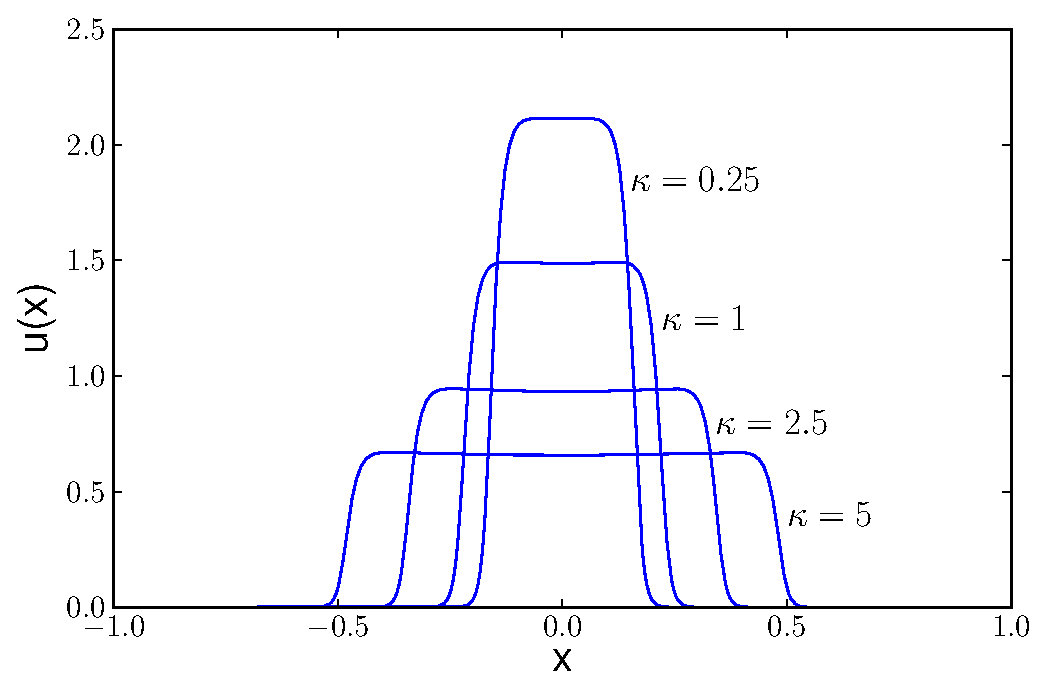
\includegraphics[width=4in]{profiles_basic_mesa_}
\caption{Mesa profiles for various values of $\kappa$, obtained by numerically solving \eqref{eqn:o-gms1}. The other parameters used are $D=10$ and $L=1$. The system was integrated using an implicit explicit scheme on a 500 point grid.}
\label{fig:mesa_profiles}
\end{center}
\end{figure}
% 
Since the solutions are no longer pulses, it is no longer possible to represent the activation term as a delta function, and generate an approximate solution via a related Greens problem (this approach applied to the Schnakenberg system can be seen in \cite{kolokolnikov_spot_2009}). The mesa solutions are no longer homoclinic solutions, instead the system can be thought of as two back-to-back heteroclinic branches. This characteristic can be exploited to obtain a first asymptotic approximation of the system. This was approach done originally in \cite{kolokolnikov_self_2007}, and is added here for the benefit of the reader.

We start by looking for an asymptotic solution near the interface $x=l$ to the steady state problem $u_t = v_t = 0$:
% 
$$
u=U_0(y) + \Ep U_1(y)+\ldots, \qquad v=V_0(y) + \Ep V_1(y)+\ldots, \qquad y=\frac{x-l}{\Ep}.
$$

To $O(1)$, since $D_u = O(\Ep^2)$, the system is
% 
\begin{equation*}
\label{eqn:order1}
\begin{split}
\begin{aligned}
	U_0'' &= U_0 - \frac{U_0^2}{V_0(1+kU_0^2)}\\
	V_0'' &= 0.
\end{aligned}
\end{split}
\end{equation*}

From the boundary conditions we have that $V_0$ is a constant. To determine its value, we use the Maxwell line condition \cite{maxwell1994}, which states that in order to have a heteroclinic connection between $x=0$ and $x=L$, there has to be a value $v_c$, such that the area under the roots of $a(u,v_c) = -u +  \frac{u^2}{v_c(1+ku^2)}$ is zero. The three roots of $a(u,v)$ occur at $u=0$ and at $u=u_{\pm}(v) = \frac{1\pm\sqrt{1-4kv^2}}{2kv}$, with $0<u_-(v)-<u_+(v)$. The non-zero roots can be expressed as $v=h(u)=\frac{u}{1+ku^2}$ for $0<v<v_m$ , with $v=v_m$ the value at which both roots coalesce. Hence, the solution to the $O(1)$ equation is $V_0=v_c$, with $v_c$ the value that satisfies the Maxwell line condition
% 
\begin{equation}
\label{eqn:maxwell}
\int_0^{u_c}a(u,v_c)=0,\qquad u_c\equiv u_+(v_c),
\end{equation}
% 
and $U_0$ the unique heteroclinic connection satisfying $U_0(-\infty)=u_+(v_c)=u_c$ and $U_0(\infty)=0$.

To $O(\Ep)$ we have the system
% 
\begin{equation*}
\label{eqn:order_eps}
\begin{split}
\begin{aligned}
	&\mathcal{L}(U_1) = U_1'' + a_u(U_0,V_0)U_1 = -a_v(U_0,V_0)V_1\\
	&V_1'' = 0.
\end{aligned}
\end{split}
\end{equation*}

The solution to the second equation is $V_1 = V_{11}y + V_{12}$. Since $\mathcal{L}(U_0')=0$, we can derive a solvability condition to determine $V_{12}$ in terms of $V_{11}$,
% 
\begin{equation*}
  \label{eqn:solvability}
  V_{12}\int_{-\infty}^{\infty}a_v(U_0,v_c)U_0'dy = V_{11}\int_{-\infty}^{\infty}a_v(U_0,v_c)yU_0'dy.
\end{equation*}

Furthermore, matching to the outer solution yields that $V_{11} = v'(l^{\pm})$.

There are two outer solutions, to the left and right of the internal layer at $x=l$, that when matched will determine the value for $v'(l^{\pm})$. The problem to the left of the layer, $0<x<l$, is
% 
\begin{equation}
  \label{eqn:left}
  D_v v'' = b(u,h(u)) = g(u),\qquad v(l)=v_c,\qquad v'(0)=0,\qquad u = u_+(v),
\end{equation}
% 
whereas the outer problem on the right side of the layer, $l<x<L$, is defined as
% 
\begin{equation}
  \label{eqn:right}
  D_v v'' = b(0,v),\qquad v(l)=v_c,\qquad v'(L)=0.
\end{equation}

Since $V_{11}$ is a constant, the matching condition is that $v'(l^-) = v'(l^+)$

Multiplying \eqref{eqn:left} by $v'=h'(u)u'$ and integrating yields the following equations for $u_x$ and $v_x$,
% 
\begin{equation*}
%   \label{eqn:left}
  \frac{dv}{dx} = -\sqrt{\frac{2F(u;u_0)}{D}},\qquad \frac{du}{dx} = -\sqrt{\frac{2F(u;u_0)}{Dh'(u)}},
\end{equation*}
% 
with $F(u;u_0) = \int_{u_0}^u g(s)h'(s)ds$. Upon integrating between $u_0=u(0)$ and $u(l)=u_c$, we obtain the following relationship:
% 
\begin{equation}
  \label{eqn:feo1}
  -\frac{l}{\sqrt{D}} = \int_{u_0}^{u_c}\frac{h'(u)}{\sqrt{2F(u;u_0)}}du = \frac{\sqrt{2F(u_c;u_0)}}{g(u_c)} + \int_{u_0}^{u_c}\frac{g'(u)}{(g(u))^2}\sqrt{2F(u;u_0)}du.
\end{equation}

The exact solution on the outer region given in \eqref{eqn:right} can be calculated analytically as 
% 
\begin{equation}
  \label{eqn:outer1}
  v(x) = v_c\left(\frac{\cosh\left[(L-x)/\sqrt{D}\right]}{\cosh\left[(L-l)/\sqrt{D}\right]}\right),\qquad v'(l^+)=-\frac{v_c}{\sqrt{D}}\tanh\left[(L-l)/\sqrt{D}\right].
\end{equation}

Finally, since $v'(l^+)=v'(l^-)$, we can solve for $l$ in \eqref{eqn:outer1} and substitute it into \eqref{eqn:feo1} to obtain the critical points at which the domain will split, as a function of the domain length and $D$:
% 
\begin{equation}
  \label{eqn:final1}
  \frac{L}{\sqrt{D}}=\tanh^{-1}\left(\frac{\sqrt{2F(u_c;u_0)}}{v_c} \right) - \frac{\sqrt{2F(u_c;u_0)}}{g(u_c)} - \int_{u_0}^{u_c}\frac{g'(u)}{(g(u))^2}\sqrt{2F(u;u_0)}du.
\end{equation}
% 

\subsection{Bifurcation analysis}

Equation \eqref{eqn:final1} provides an analytical estimate of the domain length at which splitting occurs. We want to study the splitting behaviour as the domain increases both statically (when stationary solutions are recomputed at each domain length value), and dynamically (when the domain length is a dynamic variable). We start by focusing on how solutions change numerically as the domain length increases. The boundary conditions were homogeneous Neumann, and the values of the constants were $k=2.5, \tau=1, D=1$, and $\Ep=0.02$. 

% The system given in \eqref{eqn:gms1} is solved by discretizing it in space with centred differences, and integrating the resulting ODE system with Matlab's ode15s stiff solver. 

Numerical solutions to the full 1-D problem were computed for increasing values of $L$. An initial solution was iterated until convergence for some domain length $L=L_0$; the stationary solution thus obtained then became the initial solution for an increased domain length $L=L_1$, etc. Typical solutions for 3 different values of $L$ are given in figure \ref{fig:typical}, while on the 2-mesa regime. 
% 
\begin{figure}[htb]
\begin{center}
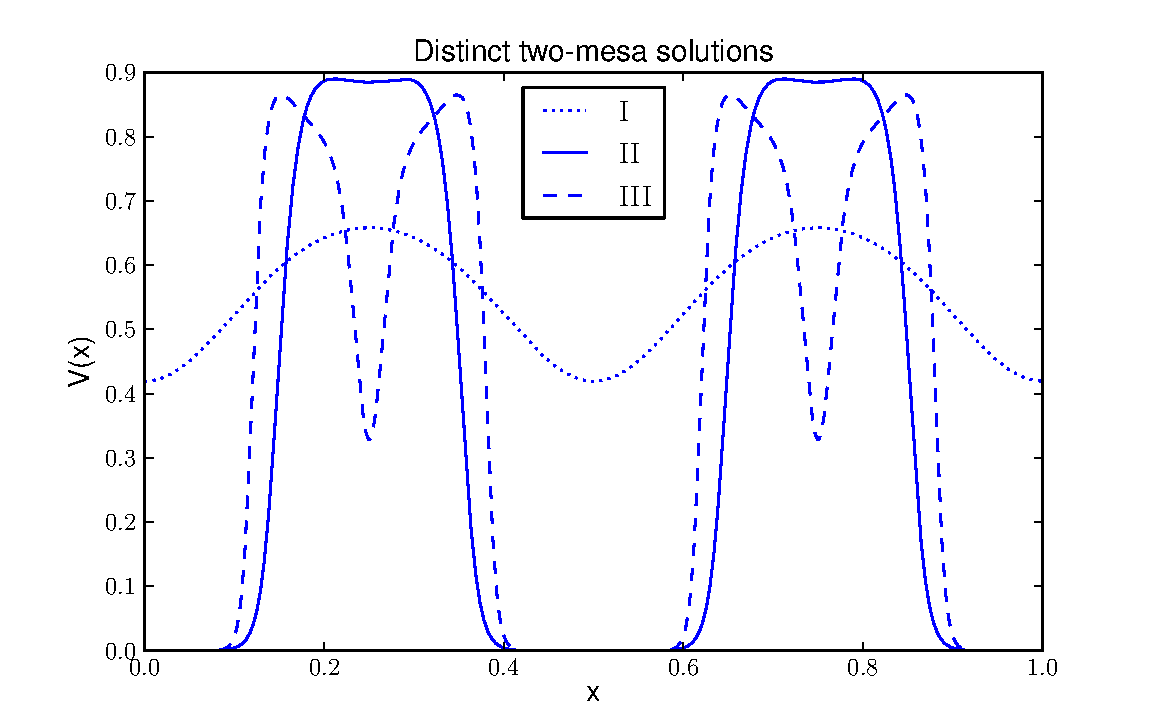
\includegraphics[width=2.5in]{typical_solutions}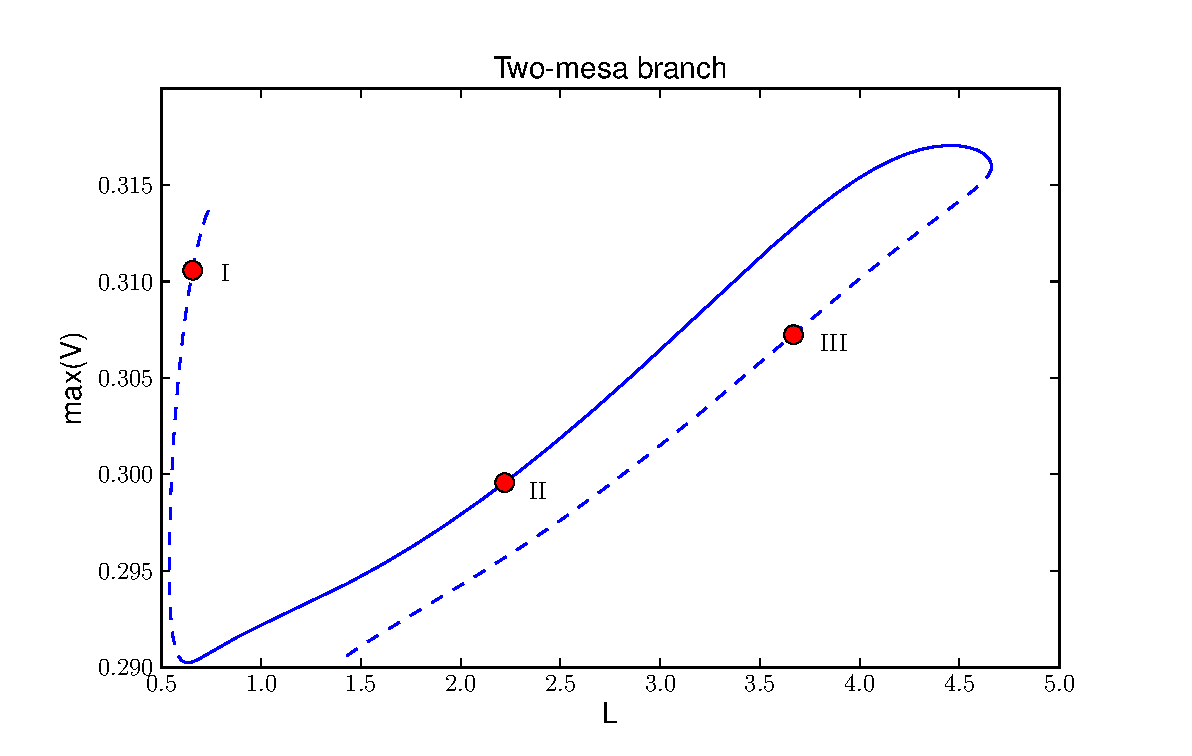
\includegraphics[width=2.5in]{two_mesa_branch}

\caption{Three distinct 2-mesa solutions to the GMS system. Solution $I$ is close to the Turing instability, $II$ is the stable mesa solution, and $III$ is the unstable solution that develops when the domain length is increased past a critical point. The image on the right is the bifurcation diagram for the branch of two-mesa solutions.}
\label{fig:typical}
\end{center}
\end{figure}
% 
The three solutions all occur for varying values of the domain length. They were all obtained through numerical continuation on the $L$ parameter. We started by obtaining a stationary solution from random initial data, and from it we used the numerical continuation package AUTO-07P \cite{doedel_auto-07p} to follow the curve of solutions for varying $L$, using $max(V)$ as the bifurcation parameter. 

Solution $I$ is essentially the leading eigenvector $\phi = A\cos(2n\pi x/L)$, first estimated through linear stability analysis, and as expected from Turing theory, unstable. Going up on the branch beyond solution $I$ leads to the homogeneous Turing solution $u=0.5603$, $v=u^2$, and traversing the branch in the other direction leads to the stable mesa branch.

Solution $II$ corresponds to the stable family of solutions, this is a characteristic mesa structure. Continuing on the branch along increasing $L$ eventually leads to a fold point, beyond which we reach the unstable branch characterized by solution $III$. Going beyond the fold point causes the solution to drop to the next branch of solutions, which will have double the number of mesas.
% 
\begin{figure}[htb]
\begin{center}
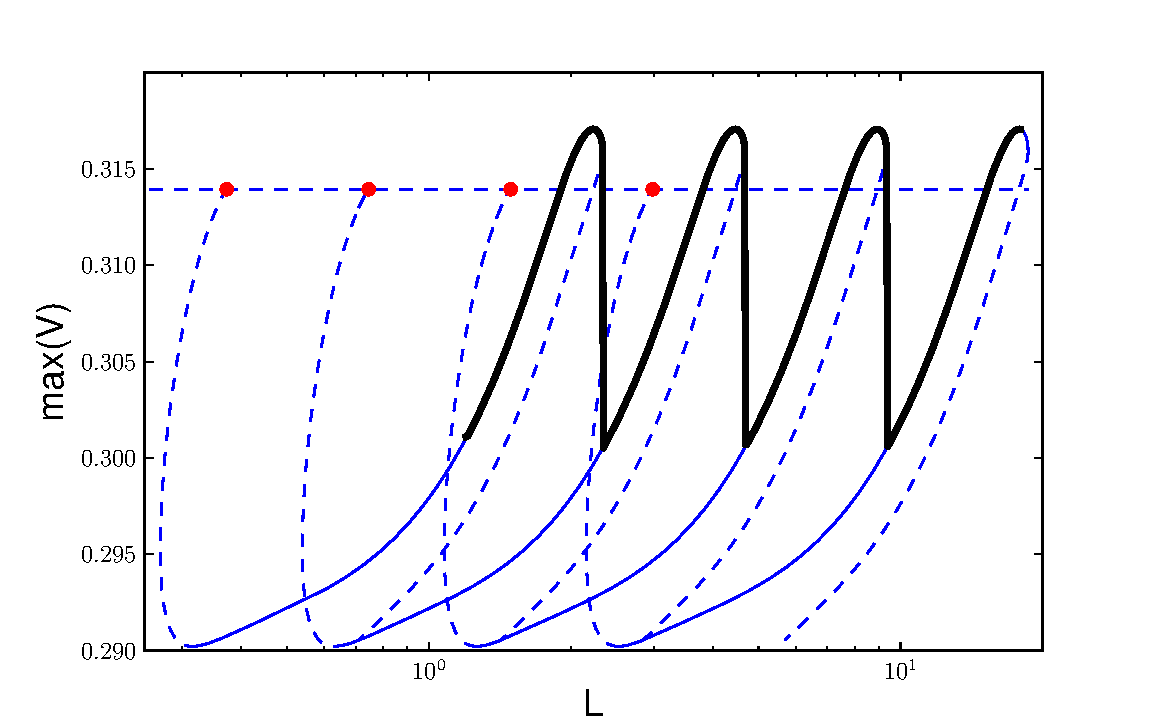
\includegraphics[width=3.5in]{one_sol_bif}
\caption{Four branches of the GMS system, with an overlay of the family of stable solutions obtained by traversing it left to right . When reaching the fold point of each branch the solutions fall to the next branch, effectively doubling the number of mesas. The upper horizontal unstable line are the unstable Turing solutions, and the red points on it are the values shown on table \ref{tab:L_turing}.}
\label{fig:one_sol}
\end{center}
\end{figure}
% 

The bifurcation diagram for one, two, four, and eight mesa solutions is given in figure \ref{fig:one_sol}. The thickest line is a stable solution that is recomputed for increasing values of $L$. It traverses the stable branches from left to right, and at each fold point it falls to the next branch, which manifests in the solutions as a doubling in the number of mesas. Since each successive branch doubles the number of mesas, the critical value $L_c$ at which the new set of mesas will split doubles with each iteration, hence $L_c(n)=L_c(1)\times 2^{n-1}$. This exponential relationship can be readily seen in the bifurcation diagram of figure \ref{fig:one_sol}, which was plotted on a logarithmic scale.

This numerical results show that there will always be a stable solution in the $(D,\tau)=O(1)$ parameter regime, for all domain lengths. The asymptotic formula \eqref{eqn:final1} provides us an estimate of the critical values $L_c(n)$ at which an $n$ mesa solution splits into $2n$ mesas. 

In order to numerically compute the value, we first found the $u_c$, $v_c$ values that satisfy the Maxwell line condition, shown in \eqref{eqn:maxwell}, via a quadrature. It was then straightforward to numerically integrate $F(u_c;u_0)$ and the third term in \eqref{eqn:final1}. 

The resulting value was $L_c = 2.1010$ for $-L<x<L$, or half that for $0<x<L$ (as shown in Figures \ref{fig:typical}, \ref{fig:one_sol}). The location of the fold point in the 1-mesa branch was then calculated by solving the full system, using $\Ep=0.002$ and $1500$ grid points. The value thus obtained was $L_c = 2.1325$.

Furthermore, the system exhibits hysteresis, traversing the bifurcation diagram left to right produces a very different picture. Traversing left to right shows the splittings occurring at the points predicted in \eqref{eqn:final1}, whereas traversing in the opposite direction results in in the solution staying in the 8-mesa branch until the left edge of the stable branch, beyond which the solution will jump either to the 4-mesa branch, or to the 2-mesa branch. In principle estimating those points should involve very similar analysis as was done in \S~\ref{section:construction}. The differences between the bifurcation structure of $u(x)$ when traversed in either direction are shown in Figure \ref{fig:up_down}.
% 
\begin{figure}[htb]
\begin{center}
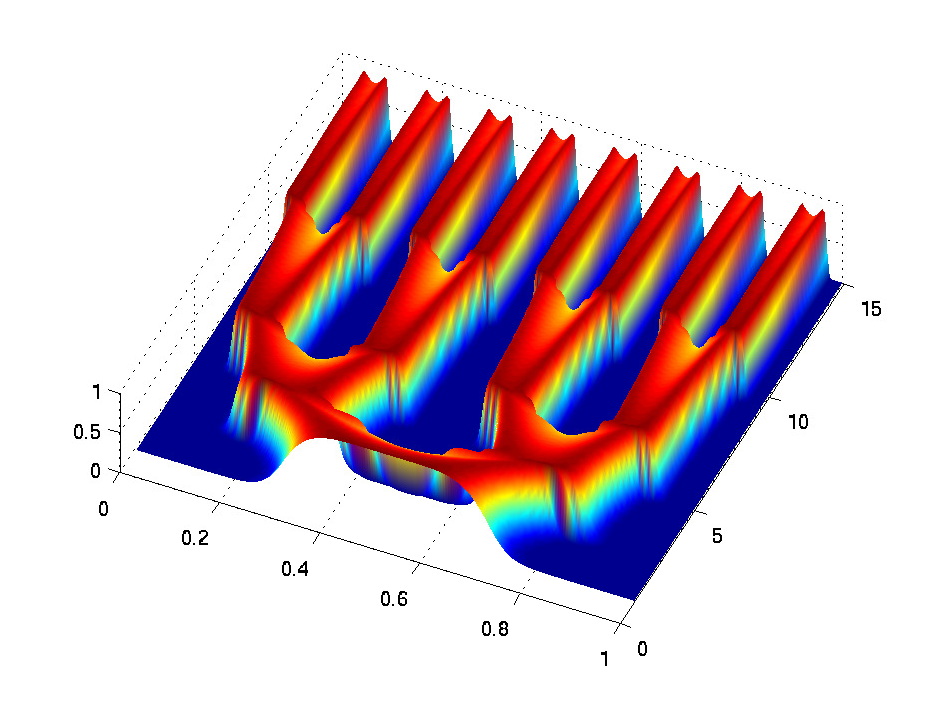
\includegraphics[width=2.5in]{full_soln_up}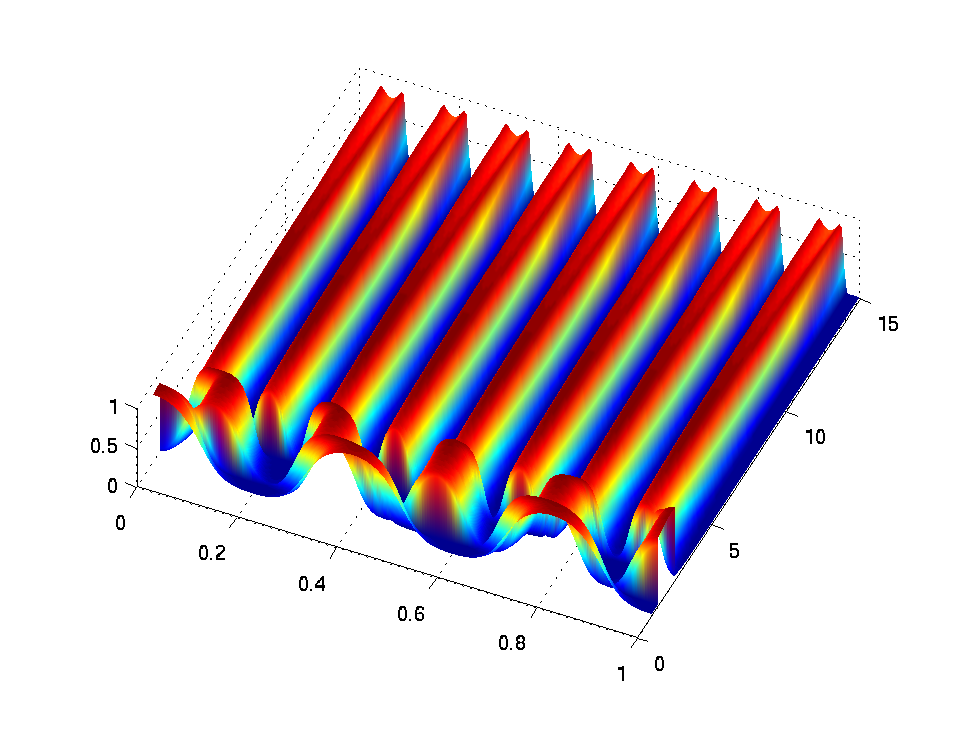
\includegraphics[width=2.5in]{full_soln_down}
\caption{The full solution curve for $u(x)$ as the bifurcation branches in Figure \ref{fig:one_sol} are traversed from left to right (image on the left), and from right to left (image on the right).}
\label{fig:up_down}
\end{center}
\end{figure}
% 

All of the work above was done with the domain length fixed; when a stable solution was attained it was used as the starting point for the next computation at a slightly changed $L$. When considering dynamically varying domains, i.e., making $L\equiv L(t)$, the system needs to be modified. A general framework on how to extend stationary equations into growing domains can be found in \cite{plaza2004growth}. The extended system for isotropic exponential growth is relatively simple, 
% 
\begin{equation*}
\label{eqn:gms_growth}
\begin{split}
\begin{aligned}
	u_t &= \frac{\Ep^2}{L^2}\De u -\rho u - u +\frac{u^2}{v(1+ku^2)} \\
	\tau v_t &= \frac{D}{L^2}\De v - \rho v - v + u^2 \\
	L_t &= \rho L,
\end{aligned}
\end{split}
\end{equation*}
% 
with $\rho$ the rate of domain growth. 

We solved the system by discretizing in space using centred differences, with second order boundary conditions, and Matlab's ode15s routine was used for time integration. The solution curves for various values of $\rho$ were obtained, and when overlapping them in the bifurcation diagram of Figure \ref{fig:one_sol} we can see a delayed bifurcation effect in the left image of Figure \ref{fig:growth}. Notice the sharp transitions of the static solutions in Figure \ref{fig:up_down}, compared to the soft dynamic transitions on the right image in Figure \ref{fig:growth}. 
% 
\begin{figure}[htb]
\begin{center}
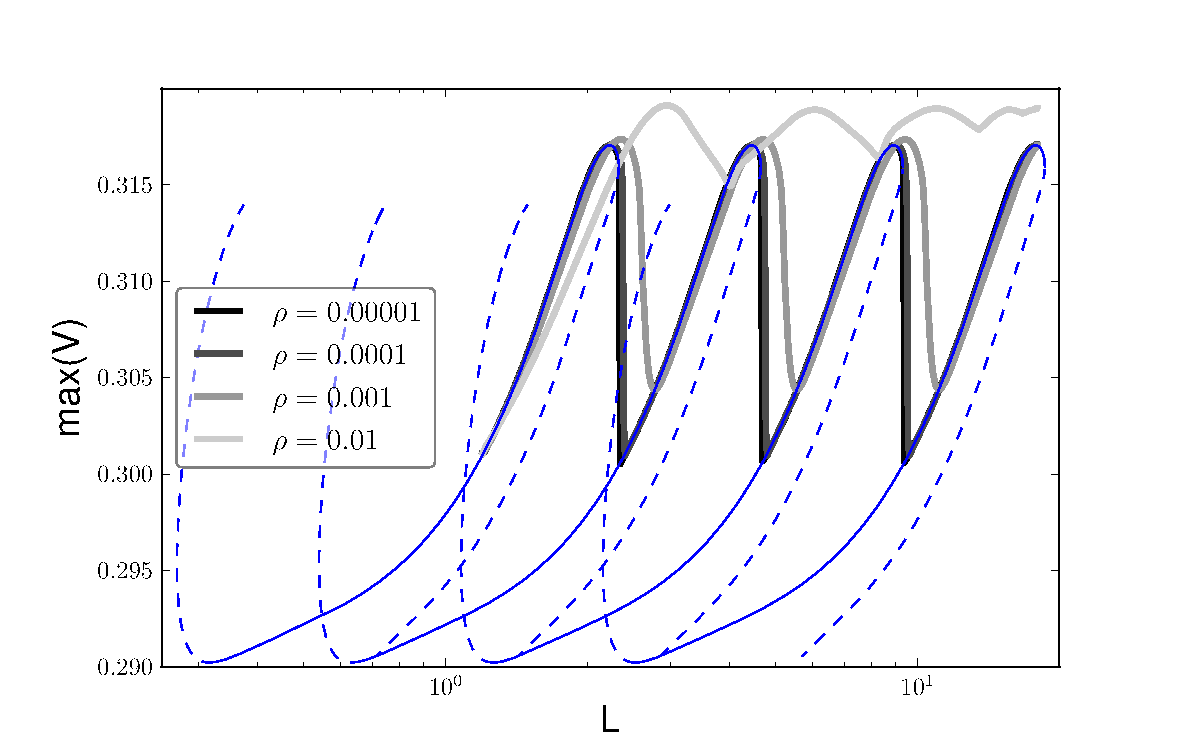
\includegraphics[width=2.5in]{all_branches}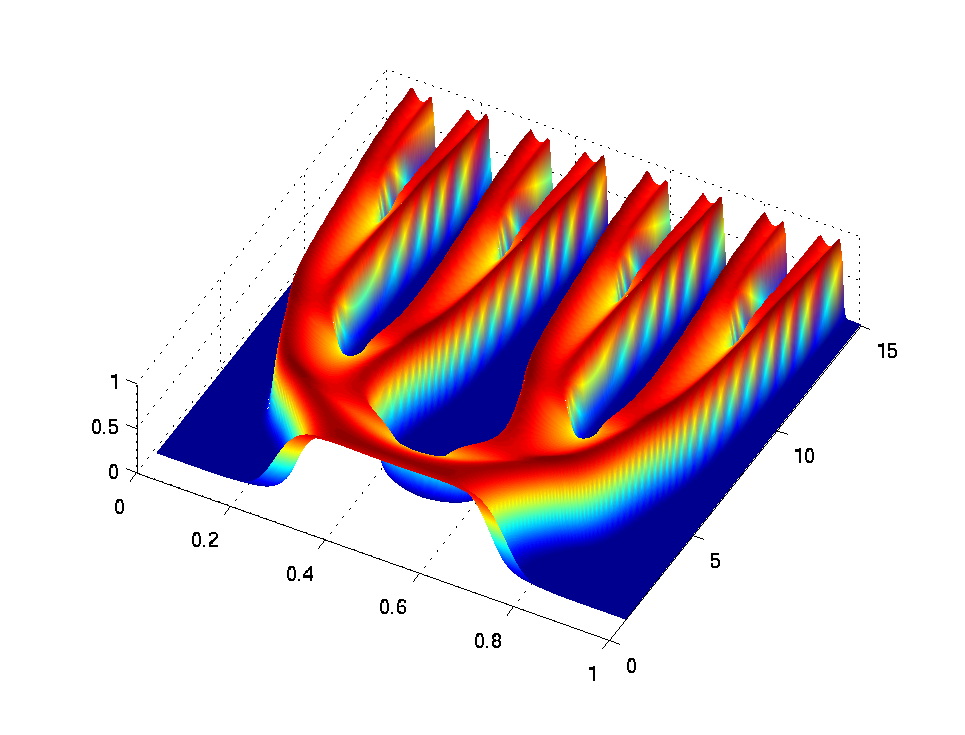
\includegraphics[width=2.5in]{growing}
\caption{Solution curves for systems with growing domains, $L(t)=e^{\rho t}$. Notice the delay in the bifurcation (jump between branches) as $\rho$ gets larger. The figure on the right shows the effect on figure \ref{fig:up_down} (left) when adding domain growth, with $\rho=0.002$.}
\label{fig:growth}
\end{center}
\end{figure}
% 

***hast aqui hoy julio 25

The stability of the branches highlighted in the above figures had to be obtained independently from the continuation software used to generate the bifurcation the diagram. The package that we used (AUTO-07P \cite{doedel_auto-07p}) is designed primarily for finite dimensional systems, and for ODE systems can easily establish stability. When extended to dealing with parabolic PDEs this capability is lost. We performed the eigenvalue analysis separately by saving the stationary solutions obtained while traversing the branches, and using them as the basis of a Taylor expansion on a perturbation to the solutions. The algorithm in AUTO utilizes non-uniform grids, so we used a spline on the output to generate a uniformly spaced grid amenable with the discrete Jacobian

Let the perturbed solutions be of the form
% 
\begin{equation}
\label{eqn:gms_eigs}
\begin{split}
\begin{aligned}
u(x) = u_s(x) + e^{\lA t}\phi(x)\\
v(x) = v_s(x) + e^{\lA t}\psi(x),
\end{aligned}
\end{split}
\end{equation}
% 
with $u_s$, $v_s$ the stationary solutions and $|u-u_s|\ll 1$, $|v-v_s|\ll 1$. Substituting into \eqref{eqn:gms1}, we get
% 
\begin{equation}
\label{eqn:gms_2}
\begin{split}
\begin{aligned}
	\lA \phi &= \Ep^2\De \phi + a_u(u_s,v_s)\phi + a_v(u_s,v_s)\psi \\
	\lA\tau \psi &= D\De \psi + b_u(u_s,v_s)\phi + b_v(u_s,v_s)\psi.
\end{aligned}
\end{split}
\end{equation}

This can be written as an eigenvalue problem in matrix form, $Aw = \lA w$, with $w = (\phi,\psi)^T$, and $A$ as
% 
\begin{equation}
\label{eqn:Amatrix}
  A =
	\begin{bmatrix}
		\Ep^2\De + a_u(u_s,v_s)& a_v(u_s,v_s) \\
		b_u(u_s,v_s)/\tau& D\De/\tau + b_v(u_s,v_s)/\tau
  \end{bmatrix}.
\end{equation}

Plotting the eigenvalue with largest real part versus the corresponding $L$ value for the stationary solutions reveals the stable and unstable manifolds in the branches. In Figure \ref{fig:eigs1} we show such a curve for the full range of stationary solutions along the 1-mesa branch. The labelling regarding stability on all the previous figures was based on this calculation, and due to the symmetry of the system, the curves for the different branches are essentially identical.
% 
\begin{figure}[htb]
\begin{center}
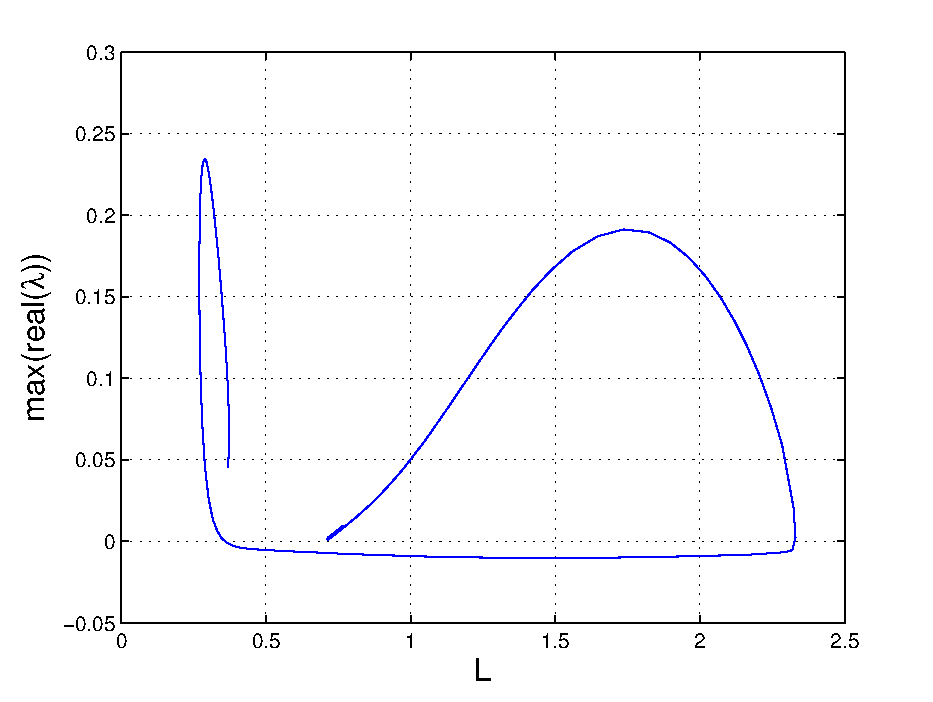
\includegraphics[width=3.5in]{eigs_1}
\caption{Stability curve of the maximum eigenvalue vs $L$ for solutions on the 1-mesa branch.}
\label{fig:eigs1}
\end{center}
\end{figure}
% 
The region in Figure \ref{fig:eigs1} where the eigenvalues have negative values is roughly a straight line of magnitude $O(\Ep)$. This was expected from the estimates done on \cite{kolokolnikov_spot_2009} (or perhaps point to latter calculations).

\subsection{Construction of the solution in the near-shadow limit}

For the near-shadow limit, $D=\DD/\Ep$, we want to construct a $K-$stripe stationary solution on $x\in[0,1]$, with $L=1/K$ the period of the solution, and $l$ the length of each individual mesa, as shown in Figure \eqref{fig:single_mesa}.
% 
\begin{figure}[htb]
\begin{center}
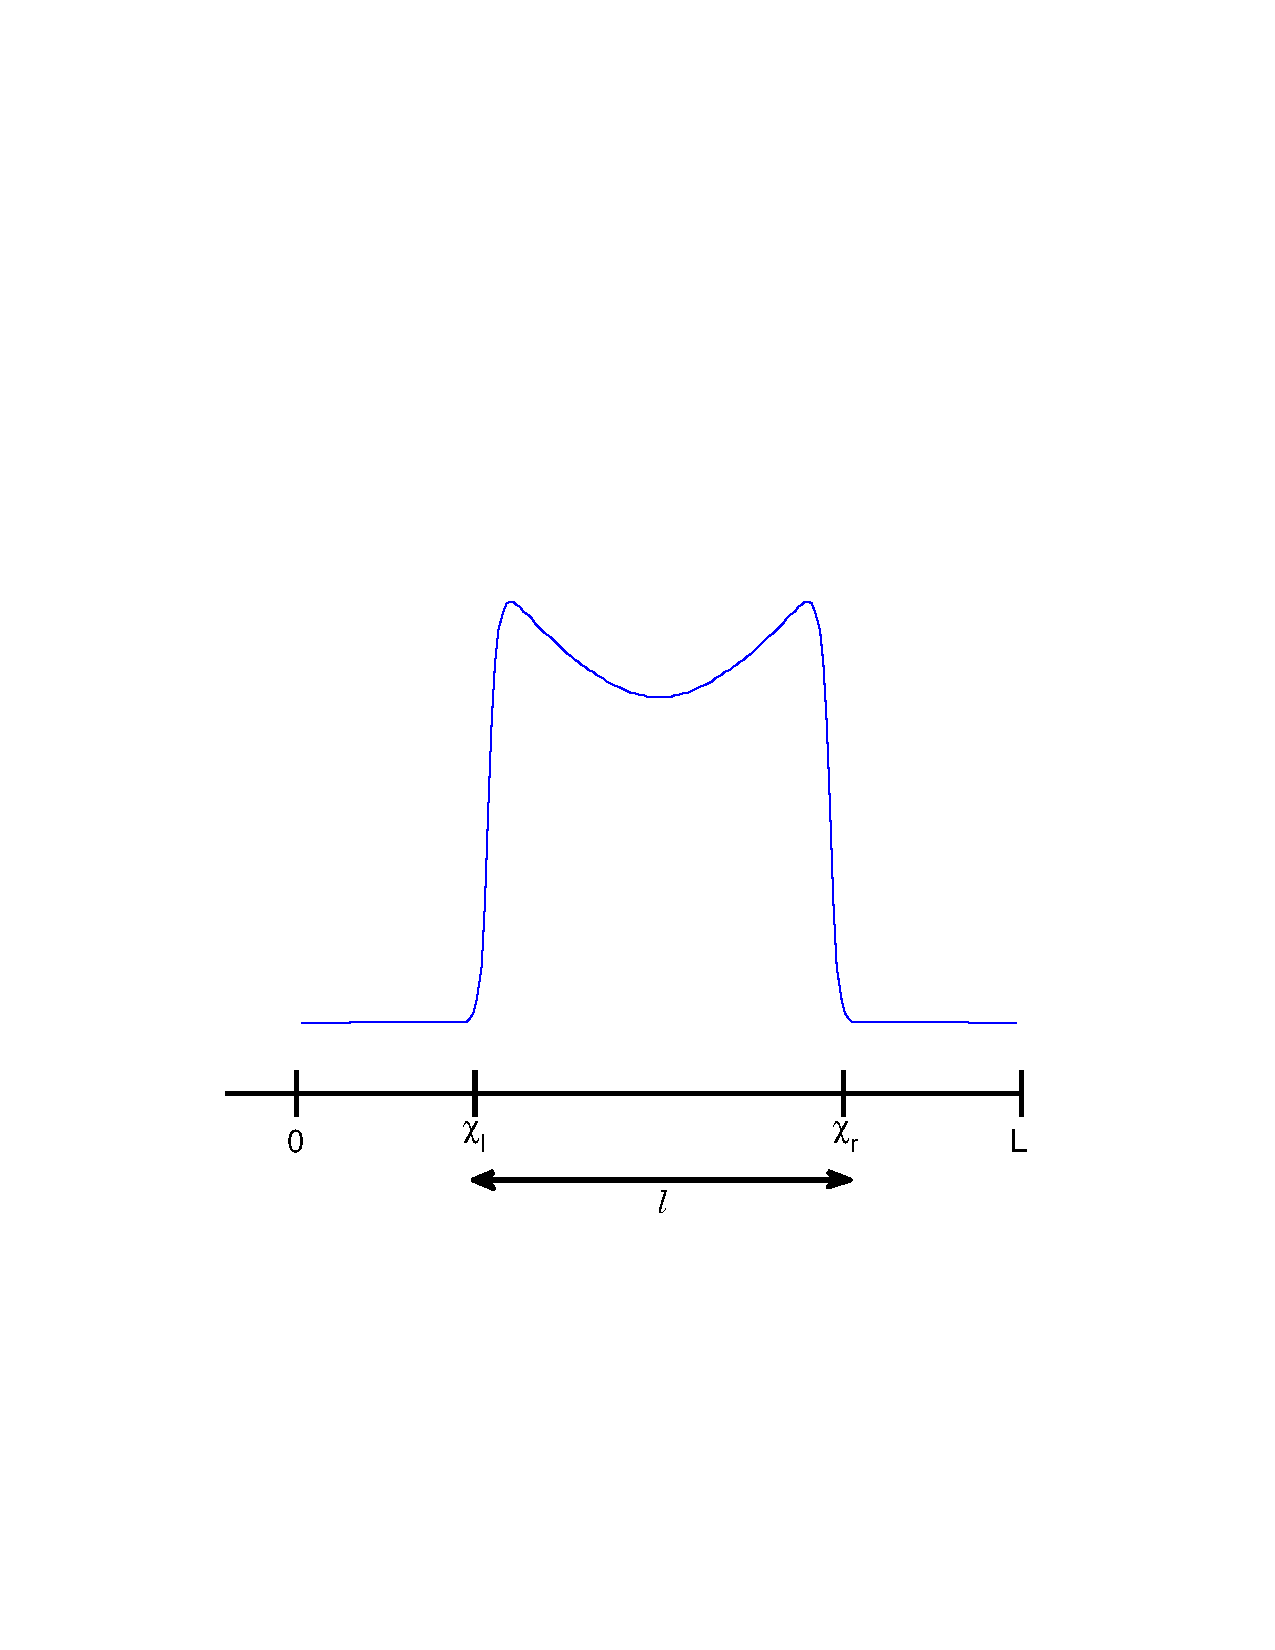
\includegraphics[width=4in]{single_mesa}
\caption{A typical mesa profile in the stationary solution $v(x)$. The left and right edges of the mesa are labelled as $\chi_l$ and $\chi_r$ respectively; and the length of the mesa section is $l$.}
\label{fig:single_mesa}
\end{center}
\end{figure}
% 
The stationary equation we want to solve is
% 
\begin{equation}
\label{eqn:o-gms_stat}
\begin{split}
\begin{aligned}
	0 &= \Ep^2 u_{xx} -u + \frac{u^2}{v(1+ku^2)},\qquad &u_x(0)=u_x(L)=0, \\
	0 &= \frac{\DD}{\Ep}v_{xx} - v + u^2,\qquad &v_x(0)=v_x(L)=0.
\end{aligned}
\end{split}
\end{equation}
% 

***did not define $g(u,v)=\frac{u^2}{v(1+ku^2)}$, as it's only used much further down the road***

To first order, we have in the $v$ equation that $v_{xx}=0$. Applying the Neumann condition, we have then that $v\sim\VV$, and the value of the constant can be estimated by integrating over the whole domain,
% 
\begin{equation}
\label{eqn:o-v_first_order}
  \VV = \frac{1}{L}\int_0^Lu^2dx.
\end{equation}
% 

In the inner region near the left boundary of the mesa we have that $v=\VV$, and we do a change of variables for $u=\VV w$ and $y=\Ep^{-1}(x-\chi_l)$. The resulting equation is
% 
\begin{equation}
\label{eqn:o-w_eqn}
  w_{yy}+f(w)=0, \qquad -\infty<y<\infty,\qquad f(w) = -w + \frac{w^2}{1+bw^2},
\end{equation}
% 
with $b = k\VV^2$. Now, we are looking for a heteroclinic connection in $u$ as the transition mechanism that generates the mesa, one for the each side of the mesa. For a heteroclinic connection to exist in \eqref{eqn:o-w_eqn}, it has to satisfy the Maxwell line condition \cite{maxwell1994}.
% 
\begin{figure}[htb]
\begin{center}
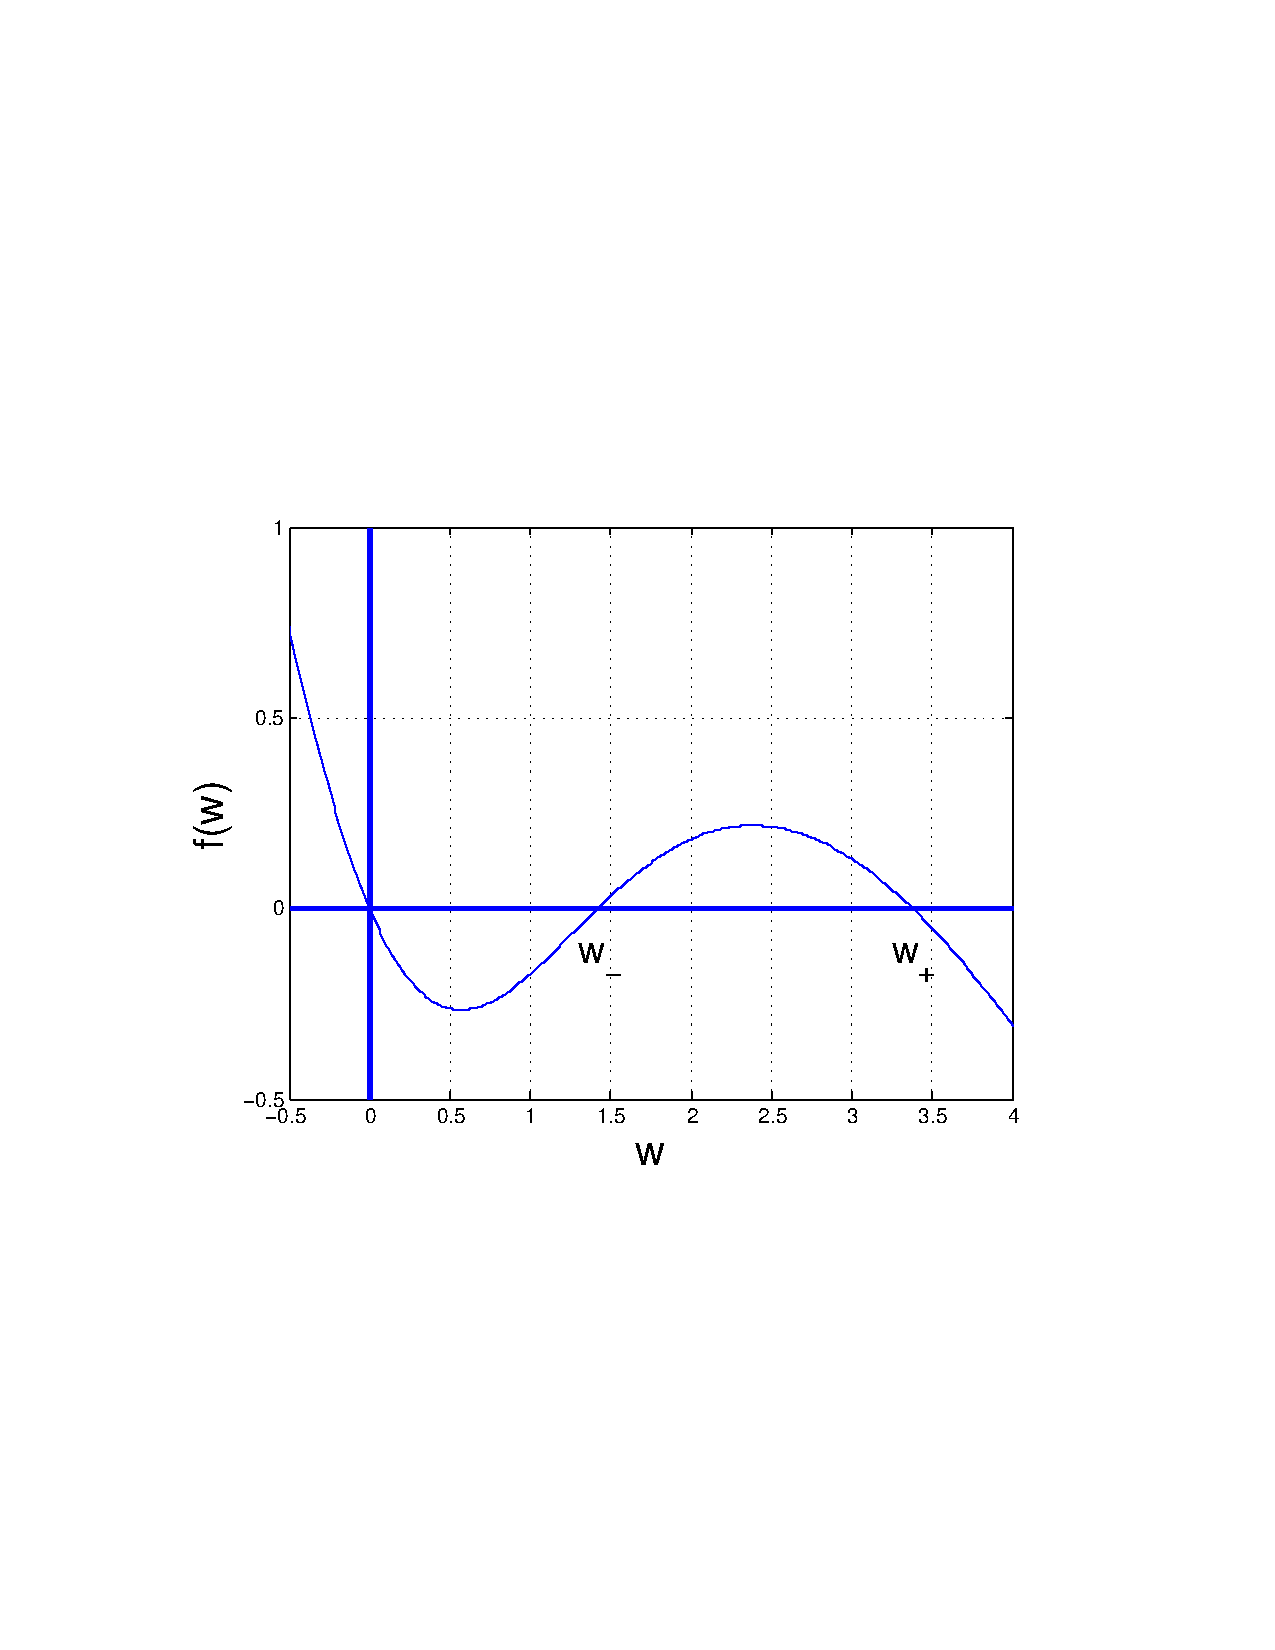
\includegraphics[width=4in]{f_of_w}
\caption{A plot of the function $f(w)$ given in \eqref{eqn:o-w_eqn}.}
\label{fig:f(w)}
\end{center}
\end{figure}
% 

The function $f(w)=0$ has zeros at $w=0$ and $w_{\pm} = \frac{1\pm\sqrt{1-4b}}{2}$, with distinct real values for $w_{\pm}$ existing in the range $0\le b<1/4$. The profile of the curve in that range can be seen in Figure \eqref{fig:f(w)}. The Maxwell line condition states that a heteroclinic connection will exist for the value $b=b_0$ such that $\int_0^{w_+} f(w)dw = 0$. Integrating $f(w)$ we get
% 
\begin{equation*}
% \label{eqn:maxwell_lc}
\begin{split}
\begin{aligned}
  \int_0^{w_+} f(w)dw &= \left.\left(-\frac{w^2}{2} + \frac{w}{b} - \frac{1}{b^{3/2}}\arctan(b^{1/2}w) \right)\right|_0^{w_+},\\
  & = -\frac{w_+^2}{2} + \frac{w_+}{b_0} - \frac{1}{b_0^{3/2}}\arctan(b_0^{1/2}w_+),
\end{aligned}
\end{split}
\end{equation*}
% 
and since we have that $b_0 = \frac{w_+-1}{w_+^2}$, the Maxwell line condition will be satisfied if
% 
\begin{equation}
\label{eqn:maxwell2}
b_0 = \frac{w_+-1}{w_+^2},\qquad \sqrt{w_+-1}(w_++1)=2w_+\arctan(\sqrt{w_+-1}).
\end{equation}

This can be solved numerically to obtain the critical values $b_0 = 0.211376$, and $w_+ = 3.295209$. (??? do a plot of numerical vs asymptotic approximation)

For use later in section \eqref{section:stability}, we need to compute
% 
$$
\beta = \int_{-\infty}^{\infty}w'^2dy
$$
% 

We multiply \eqref{eqn:o-w_eqn} by $w'$ to get 
% 
\begin{equation*}
  \frac{d}{dy}\left(\frac{w'^2}{2} \right)=\frac{d}{dy}\mathcal{F}(w)\qquad\rightarrow\qquad w'^2 = 2\mathcal{F},
\end{equation*}
% 
with $\mathcal{F} = \int_0^wf(s)ds$. We then get
% 
\begin{equation}
\label{eqn:o-beta}
  \beta = \int_{-\infty}^{\infty}w'^2dy = \int_{0}^{w_+}w'^2\frac{1}{w'} dw = \int_{0}^{w_+}\sqrt{2\mathcal{F}(w)}dw.
\end{equation}
% 

This can be numerically calculated using the previously computed value for $w_+$, to get $\beta\sim1.49882$.

Linearizing around $w=0$ for $y\rightarrow -\infty$, and for $w=w_+$ for $y\rightarrow \infty$, we get that for $b=b_0$ we have a heteroclinic solution 
% 
\begin{equation*}
% \label{eqn:hetero}
\begin{split}
\begin{aligned}
  &w''+f(w)=0,\qquad &-\infty<y&<\infty,\qquad f(w) = -w + \frac{w^2}{1+b_0w^2},\\
  &w\sim d_-e^y,\qquad &&\mathrm{as}\hspace{2pt}y\rightarrow -\infty,\\
  &w\sim w_+ - d_+e^{-\nu_+y},\qquad&&\mathrm{as}\hspace{2pt}y\rightarrow \infty,
\end{aligned}
\end{split}
\end{equation*}
% 
for $\nu_+ = \sqrt{1-2/w_+}$. By translation we take $w(0)=w_+/2$, in order to have uniqueness.

A full mesa solution will consist of two back-to-back heteroclinic curves, and can be constructed as
% 
\begin{equation*}
  u\sim \VV[w_l + w_r - w_+],\qquad  \textrm{with }w_l\sim w\left(\frac{x-\chi_l}{\Ep}\right),\qquad w_r\sim w\left(\frac{\chi_r-x}{\Ep}\right).
\end{equation*}
% 

Integrating \eqref{eqn:o-v_first_order}, we get that to first order $\VV\sim\frac{1}{L}\VV^2w_+^2l$, with $l=\chi_r-\chi_r$ the width of the mesa. We then have
% 
\begin{equation*}
  \VV w_+^2\sim\frac{L}{l} + O(\Ep),\qquad l\sim\frac{L\sqrt{k}}{\sqrt{b_0}w_+^2}<L,
\end{equation*}
% 
therefore a necessary condition for a $K-$stripe solution to exist is that 
% 
\begin{equation*}
  \frac{\sqrt{k}}{\sqrt{b_0}w_+^2}<1.
\end{equation*}
% 

To refine the solution, it is necessary to further expand $u(x)$ and $v(x)$. In the outer region we expand $u$ and $v$ as
$$
v\sim \VV + \Ep v_1 + \Ep^2 h_2 + \cdots.
$$

Since outside of the mesa $u$ is exponentially small, and in the plateau region $u\sim\VV w_+ + O(\Ep)$, by substituting into \eqref{eqn:o-gms_stat}, we get that
% 
\begin{equation}
\label{eqn:o-v1}
	\begin{split}
	\DD v_{1,xx}
   = \left\{
	\begin{matrix}
		\VV& \mathrm{for}\hspace{2pt}0< x<\chi_l \\
		\VV(1-\VV w_+^2) = \VV(1-L/l)& \mathrm{for}\hspace{2pt}\chi_l< x<\chi_r\\
		\VV& \mathrm{for}\hspace{2pt}\chi_r<x<L
	\end{matrix}\right.
	\end{split}
\end{equation}
% 
with $v_{1,x}(0) = v_{1,x}(L) = 0$. In order to find the conditions on $v_1$ at the transition layers $\chi_l$ and $\chi_r$, we expand $u$ as $u\sim\VV w_+ + \Ep\UU_1 + ...$ on $\chi_l<x<\chi_r$.

Substituting into \eqref{eqn:o-gms_stat}, we get that 
\[
-\UU_1 + g_u(\VV w_+,\VV)\UU_1 + g_v(\VV w_+,\VV)v_1 = 0.
\]

Since $1+b_0w_+^2 = w_+$, the linearization terms simplify to
% 
\begin{equation}
\label{eqn:derivs}
\begin{split}
\begin{aligned}
  g_u(\VV w_+,\VV) = \frac{2w_+}{(1+b_0w_+^2)^2} = \frac{2}{w_+},\\
  g_v(\VV w_+,\VV) = \frac{-w_+^2}{1+b_0w_+^2} = -w_+,
\end{aligned}
\end{split}
\end{equation}
% 
and this yields
$$
-\UU_1 + \frac{2}{w_+}\UU_1 - w_+v_1 = 0,\qquad \Rightarrow \qquad \UU_1 = \frac{w_+^2}{2-w_+}v_1.
$$

We now expand $u$ and $v$ near the $x=\chi_l$ $(y=\Ep^{-1}(x-\chi_l))$ as
% 
\begin{equation*}
  u = u_0 + \Ep u_1 + \Ep^2 u_2+ \cdots,\qquad v = \VV + \Ep\VV_1 + \Ep^2\VV_2+\cdots,
\end{equation*}
% 
with $u_0 = \VV w_+$. Substituting into \eqref{eqn:o-gms_stat}, the $O(\Ep)$ system is
% 
\begin{equation}
\label{eqn:ord_epsilon}
\begin{split}
\begin{aligned}
  \LL u_1:&\equiv u_1''-u_1 + g_u(u_0,\VV)u_1 = -g_v(u_0,\VV)\VV_1 \\
  \VV_1'' &= 0.
\end{aligned}
\end{split}
\end{equation}
% 

For $\VV_1$ we get that $\VV_1 = \VV_{10} + \VV_{11}y$. We have that $\LL a_0' = 0$.

The solvability condition on \eqref{eqn:ord_epsilon} is then that 
% 
\begin{equation}
\label{eqn:solvab}
\begin{split}
\begin{aligned}
\int_{-\infty}^{\infty}g_v(u_0,\VV)\VV_1u_0'dy = \int_{-\infty}^{\infty}\frac{w^2}{1+bw^2}w'\VV_1dy = 0.
\end{aligned}
\end{split}
\end{equation}
% 

Substituting in $\VV_1 = \VV_{10} + \VV_{11}y$, the condition from \eqref{eqn:solvab} implies that
% 
\begin{equation*}
% \label{eqn:solvab2}
\begin{split}
\begin{aligned}
\VV_{10}\int_{-\infty}^{\infty}\frac{w^2w'}{1+bw^2}dy + \VV_{11}\int_{-\infty}^{\infty}\frac{w^2w'y}{1+bw^2}dy = 0.
\end{aligned}
\end{split}
\end{equation*}
% 

Since $\VV_1 = O(\Ep)$, $\VV_{11}$ has to be zero, as otherwise for $|y|\gg 1$ we would have $\VV_1 = O(1)$. Consequently, $\VV_{10}$ also has to be zero, and the conclusion is that $\VV_1=0$. We have then that $\LL u_1 = 0$, and therefore we also have $u_1 = 0$

This result yields that 
% 
\begin{equation*}
  v_1(\chi_l)  = v_1(\chi_r) = 0,
\end{equation*}
% 
and now we have enough conditions to solve uniquely for $v_1$.

Using the fact that $\chi_r-\chi_l = l$, and that $\VV w_+^2 = L/l$, the full solution to \eqref{eqn:o-v1} is
% 
\begin{equation*}
% \label{eqn:v1_full}
	\begin{split}
	v_1
   = \left\{
	\begin{matrix}
		\frac{\VV}{2\DD}(x^2-\chi_l^2)& \mathrm{for}\hspace{2pt}0< x<\chi_l \\
		\frac{\VV(l-L)}{2\DD l}[(x-\chi_l)^2 - l(x-\chi_l)]& \mathrm{for}\hspace{2pt}\chi_l< x<\chi_r\\
		\frac{\VV}{2\DD}[(L-x)^2-(L-\chi_r)^2]& \mathrm{for}\hspace{2pt}\chi_r<x<L
	\end{matrix}\right.
	\end{split}
\end{equation*}
% 

It is possible now to calculate $v_{1,x}$ close to the transition layers. We have
% 
\begin{equation}
\label{eqn:v1x}
\begin{split}
\begin{aligned}
  v_{1,x}(\chi_l^-) = \frac{\VV\chi_l}{\DD},\qquad &v_{1,x}(\chi_l^+) = \frac{\VV(L-l)}{2\DD},\\
  v_{1,x}(\chi_r^-) = -\frac{\VV(L-l)}{2\DD},\qquad &v_{1,x}(\chi_r^+) = -\frac{\VV(L-\chi_r)}{\DD},\\
\end{aligned}
\end{split}
\end{equation}
% 

% From equilibrium theory (ref ???), we have that $v_{1,x}(\chi_l^-) = v_{1,x}(\chi_l^+)$, as well as $v_{1,x}(\chi_r^-) = v_{1,x}(\chi_r^+)$. This yields that $\chi_l = \frac{L-l}{2}$, and $\chi_r = \frac{L+l}{2}$.

This suggests that there is a term to next order, as $\VV_2\sim v_{1,x}(\chi_l)$. Expanding to next order in the inner region, as $u = u_0 + \Ep^2u_2$ and $v = \VV + \Ep^2\VV_2$, and defining $g_0(w) = \frac{w^2}{1+b_0w^2}$, we have the system
% 
\begin{equation*}
% \label{eqn:solva2}
\begin{split}
\begin{aligned}
  \LL u_2 =  u_2'' - u_2 + g_0'(w)u_2 = g_0(w)\VV_2,\\
  \VV_2'' = 0.
\end{aligned}
\end{split}
\end{equation*}
% 

We have then that $\VV_2 = \VV_{20} + y\VV_{21}$. 

We can derive a solvability condition from $\LL u_2 = g_0(w)\VV_2$, since $\LL w'=0$. We get
% 
\begin{equation*}
  \int_{-\infty}^{\infty}\VV_2g_0(w)w'dy = \int_{-\infty}^{\infty}(\VV_{20} + y\VV_{21})g_0(w)w'dy = 0,
\end{equation*}
% 

We can now match the inner solution to the outer solution evaluated at the interface, to determine $\VV_{20}$ and $\VV_{21}$. We get that
% 
\begin{equation*}
  \VV + \Ep^2(\VV_{20} + y\VV_{21}) + \cdots = \VV + \Ep v_1(\chi_l) + \Ep v_{1,x}(\chi_l^-)(x-\chi_l) + \Ep^2v_2(\chi_l)+\cdots
\end{equation*}
% 

From this we can conclude that $\VV_{21} = v_{1,x}(\chi_l^-)$, and that $\VV_{20} = v_2(\chi_l)$. This last value, for both the inner and outer solutions, can be calculated from the solvability condition given that we now know $\VV_{21}$. 

Furthermore, repeating the matching procedure with $x\rightarrow \chi_l^+$ yields the same value, as the outer solution has no ambiguity. From this we get that $v_{1,x}(\chi_l^+) = v_{1,x}(\chi_l^-)$. Repeating the procedure yet again at the right boundary $\chi_r$, we get the same result, i.e., $v_{1,x}(\chi_r^+) = v_{1,x}(\chi_r^-)$. Since we already knew from \eqref{eqn:v1x} that $v_{1,x}(\chi_l^+) = - v_{1,x}(\chi_r^-)$, we can solve for $\chi_l$ and $\chi_r$ to get that the position of the boundaries of the mesa on $[0,L]$ are
% 
$$
  \chi_l = \frac{L-l}{2}, \qquad \chi_r = \frac{L+l}{2},
$$
% 
with $l$ the length of the plateau. A corollary from this result is that that stationary mesa solutions have to be centred.

We can find a second solvability condition that will be of use later on. Differentiating with respect to $y$, we have
% 
\begin{equation*}
  \LL u_2' = -g_0''(w)u_2w' + g_0(w)\VV_2' + g_0'(w)\VV_2w',
\end{equation*}
% 
and using the fact that $\LL w'=0$, the solvability condition we get is
% 
\begin{equation}
\label{eqn:solva1}
\begin{split}
\begin{aligned}
  -\VV_{21}\int_{-\infty}^{\infty}g_0(w)w'dy = \int_{-\infty}^{\infty}(g_0'(w)\VV_2 - g_0''(w)u_2)w'^2dy,\\
  v_{1,x}(\chi_r)\int_{-\infty}^{\infty}g_0(w)w'dy = \int_{-\infty}^{\infty}(g_0'(w)\VV_2 - g_0''(w)u_2)w'^2dy,
\end{aligned}
\end{split}
\end{equation}
% 
since $\VV_2' = \VV_{21} = -v_{1,x}(\chi_r)$.


\subsection{\label{section:stability}Stability in the near-shadow limit to perturbations in the y direction}

We assume that the solutions exist in a rectangular domain $[0,1]\times[0,d_0]$, with Neumann boundary conditions on all sides. We introduce a perturbation on the equilibrium solution $(u_e,v_e)$ of the form
% 
\begin{equation*}
  u = u_e + e^{\lA timy}\phi(x),\qquad v = v_e + e^{\lA timy}\psi(x); \qquad m = \frac{k\pi}{d_0},k=1,2,\ldots,
\end{equation*}
%
with $|\phi(x)|\ll1$, and $|\psi(x)|\ll1$.

Substituting into \eqref{eqn:o-gms1}, we get the following eigenvalue problem
%
\begin{subequations}
\begin{align}
\label{eqn:eigen_gms1}
  \bar{\lA}\phi = \LL_{\Ep}\phi + g_v(u_e,v_e)\psi &= \Ep^2\phi_{xx} - \phi + g_u(u_e,v_e)\phi + g_v(u_e,v_e)\psi,\\
\label{eqn:eigen_gms2}
  \frac{\Ep}{\DD}(1+\tau\lA)\psi &= \psi_{xx} - m^2\psi + \frac{2\Ep}{\DD}u_e\phi,
\end{align}
\end{subequations}
% 
with $\bar{\lA} = \lA + \Ep^2m^2$, and Neumann conditions $\phi_x(0)=\phi_x(1)=\psi_x(0)=\psi_x(1)=0$.

As shown in \eqref{eqn:derivs}, in the plateau region we have that $g_u(u_e,v_e) = 2/w_+$, and $g_v(u_e,v_e) = -w_+$. Substituting into \eqref{eqn:eigen_gms1}, we have that, to first order, when $\bar{\lA}\ll 1$ (???), the asymptotic form of $\phi$ on the plateau region is 
% 
\begin{equation*}
  \phi = \mu\psi,\qquad \textrm{with  }\mu \equiv \frac{w_+^2}{2-w_+},\qquad \chi_l<x<\chi_r.
\end{equation*}
% 
Outside of the plateau region $\phi$ is asymptotically small, therefore near the transition layers located at $\chi_l,\chi_r$, $\phi$ is proportional to the derivative $w'$ of the heteroclinic connection. We have then the following asymptotic form for $\phi$
% 
\begin{equation*}
% \label{eqn:phi_asy2}
	\begin{split}
	\phi
   \sim \left\{
	\begin{matrix}
		c_{li}(w'(\Ep^{-1}(x-\chi_{li}))+O(\Ep))& \mathrm{for}\hspace{2pt} x\sim\chi_{li}& \\
		c_{ri}(w'(\Ep^{-1}(\chi_{ri}-x))+O(\Ep))& \mathrm{for}\hspace{2pt} x\sim\chi_{ri}& \\
		\phi_i = \mu\psi& \mathrm{for}\hspace{2pt}x\in(\chi_{li},\chi_{ri}),&i=1,\hdots,K,
	\end{matrix}\right.
	\end{split}
\end{equation*}
% 
with the constants $c_{li},c_{ri}$ to be found.

Since $\phi$ is localized near the transition layers, we can estimate it in the sense of distributions, approximating $u_e$ as $u_e\sim\VV w$
% 
\begin{equation*}
\begin{split}
\begin{aligned}
  \frac{2\Ep u_e\phi}{\DD}&\sim \frac{2\Ep^2\VV c_l}{\DD}\int_{-\infty}^{\infty}w_lw_l'dy\dE(x-x_l) +...\\ 
  &\qquad+\frac{2\Ep^2\VV c_r}{\DD}\int_{-\infty}^{\infty}w_rw_r'dy\dE(x-x_r) + \frac{2\Ep\VV}{\DD}w_+\mu\psi H_{[\chi_l,\chi_r]},
\end{aligned}
\end{split}
\end{equation*}
% 
with $H_{[\chi_l,\chi_r]} = 1$ on $x\in (\chi_l,\chi_r)$, and zero elsewhere.

This then yields
% 
\begin{equation*}
% \label{eqn:phi_main}
\begin{split}
\begin{aligned}
\frac{2\Ep u_e\phi}{\DD}&\sim \frac{\Ep^2\VV c_lw_+^2}{\DD}\dE(x-x_l) +\frac{\Ep^2\VV c_rw_+^2}{\DD}\dE(x-x_r) + \frac{2\Ep\VV w_+\mu\psi H}{\DD}
\end{aligned}
\end{split}
\end{equation*}
% 
Substituting into \eqref{eqn:eigen_gms2}, we get that $\psi$ satisfies
% 
\begin{equation}
\label{eqn:phi_main2}
\begin{split}
\begin{aligned}
\psi_{xx}-\tH^2\psi = -\frac{\Ep^2\VV w_+^2}{\DD}\left[\sum_i(c_{li}\dE(x-\chi_{li}) + c_{ri}\dE(x-\chi_{ri})) \right],
\end{aligned}
\end{split}
\end{equation}
% 
with $\tH$ the piecewise constant function
% 
\begin{equation}
\label{eqn:phi_asym}
	\begin{split}
	\tH
   = \left\{
	\begin{matrix}
		\tH_-\equiv\left(m^2+\frac{\Ep(1+\tau\lA)}{\DD}\right)^{1/2},& \mathrm{for}\hspace{2pt} x\notin\cup_{i=1}^K[\chi_{li},\chi_{ri}]\\
		\tH_+\equiv\left(m^2+\frac{\Ep(1+\tau\lA)}{\DD}\left(1+\frac{2w_+}{l(w_+-2)} \right)\right)^{1/2},& \mathrm{for}\hspace{2pt} x\in\cup_{i=1}^K[\chi_{li},\chi_{ri}]
	\end{matrix}\right.
	\end{split}
\end{equation}
% 

Since $w'$ is localized, we can define $w'_{li}=w'(x-\chi_{li})$ and $w'_{ri}=w'(\chi_{ri}-x)$, and multiply it into \eqref{eqn:eigen_gms1}, to obtain the matrix eigenvalue problem
% 
\begin{equation}
\label{eqn:matrix_eigen_l}
  c_{li}(w'_{li},\LL_{\Ep}w'_{li}) + (w'_{li},g_v(u_e,v_e)\psi) = c_{li}\bar{\lA}(w'_{li},w'_{li}),
\end{equation}
% 
and similarly
% 
\begin{equation}
\label{eqn:matrix_eigen_r}
  c_{ri}(w'_{ri},\LL_{\Ep}w'_{ri}) + (w'_{ri},g_v(u_e,v_e)\psi) = c_{ri}\bar{\lA}(w'_{ri},w'_{ri}),
\end{equation}
% 
where $(f,g) = \int_0^1fgdx$.

The second term in \eqref{eqn:matrix_eigen_l} and \eqref{eqn:matrix_eigen_r} can be readily estimated, using the fact that $w''-w = g_0(w)$, and that $g_v=-g_0$, as
% 
\begin{equation*}
\begin{split}
\begin{aligned}
% \label{eqn:2ndterml}
  (w'_{li},g_v(u_e,v_e)\psi) = \int_0^1 w_{li}'\psi g_v(u_e,v_e)dx  =-\Ep\psi(\chi_l)\int_{-\infty}^{\infty}w'g_0(w)dy  \\
  =-\Ep\psi(\chi_l)\int_{-\infty}^{\infty}w'(w''-w)dy = -\Ep\psi(\chi_l)\frac{w_+^2}{2},
\end{aligned}
\end{split}
\end{equation*}
% 
and similarly, 
% 
\begin{equation*}
\begin{split}
\begin{aligned}
% \label{eqn:2ndtermr}
  (w'_{ri},g_h(u_e,v_e)\psi) = -\Ep\psi(\chi_r)\frac{w_+^2}{2}.
\end{aligned}
\end{split}
\end{equation*}
% 

The third term can be estimated straight from the definition of $\beta$ in \eqref{eqn:o-beta}. We get
% 
\begin{equation*}
\begin{split}
\begin{aligned}
% \label{eqn:third term}
  (w'_{li},w'_{li})) \sim \Ep\int_{-\infty}^{\infty}(w')^2dy = \Ep\beta.
\end{aligned}
\end{split}
\end{equation*}
% 

The first term can be estimated using some of the results previously obtained. We have that 
% 
\begin{equation*}
  \LL_{\Ep}w_l'=(w_l')''-w_l'+g_u(u_e,v_e)w_l'.
\end{equation*}
%

We can approximate $g_u(u_e,v_e)$ as 
% 
\begin{equation*}
g_u(u_e,v_e)\sim g_u(w\VV,\VV) + \Ep^2(g_{uu}(w\VV,\VV) + g_{uv}(w\VV,\VV))+\cdots.
\end{equation*}
% 
The derivatives can be related to $g_0(w) = \frac{w^2}{1+b_0w^2}$ in the following way:
% 
\begin{equation*}
\begin{split}
\begin{aligned}
% \label{eqn:derivs_g}
  g_u(u,v)&=\frac{2u}{v(1+ku^2)^2}\sim\frac{2w}{(1+b_0w^2)^2}=g_0'(w),\\
  g_{uu}(u,v)&=\frac{1}{v}\frac{2-6ku^2}{(1+ku^2)^3}\sim\frac{1}{\VV}\frac{2-6b_0w^2}{(1+b_0w^2)^3}=\frac{1}{\VV}g_0''(w),\\
  g_{uv}(u,v)&=-\frac{2u}{v^2(1+ku^2)^2}\sim-\frac{2w}{\VV(1+b_0w^2)^2}=-\frac{1}{\VV}g_0'(w).
\end{aligned}
\end{split}
\end{equation*}
% 

Substituting them in, we get
% 
\begin{equation*}
\begin{split}
\begin{aligned}
  g_u(u_e,v_e)\sim g_0'(w)+\frac{\Ep^2}{\VV}(g_0''(w)u_2 - g_0'(w)\VV_2)+\cdots,\\
  \LL_{\Ep}w_{li}' \sim \frac{\Ep^2}{\VV}(g_0''(w_{li})u_2 - g_0'(w_{li})\VV_2)w_{li}'.
\end{aligned}
\end{split}
\end{equation*}
%

We then get for the first term
% 
\begin{equation*}
\begin{split}
\begin{aligned}
  (w'_{li},\LL_{\Ep}w'_{li}) &\sim \frac{\Ep^2}{\VV}\int_0^1\left(g_0''(w_{li})u_2 - g_0'(w_{li})\VV_2 \right)w_{li}'^2dx \\
  &\qquad= \frac{\Ep^3}{\VV}\int_{-\infty}^{\infty}\left(g_0''(w_{li})u_2 - g_0'(w_{li})\VV_2 \right)w_{li}'^2dy
\end{aligned}
\end{split}
\end{equation*}
% 

Using the solvability condition in \eqref{eqn:solva1}, 
% 
\begin{equation*}
\begin{split}
\begin{aligned}
  \VV_2'\int_{-\infty}^{\infty}g_0(w)w'dy = \int_{-\infty}^{\infty}(g_0'(w)\VV_2 - g_0''(w)u_2)w'^2dy,
\end{aligned}
\end{split}
\end{equation*}
% 
we get
% 
\begin{equation*}
\begin{split}
\begin{aligned}
  (w'_{li},\LL_{\Ep}w'_{li}) &\sim \frac{\Ep^3}{\VV}\VV_2'\int_{-\infty}^{\infty}g_0(w)w'dy = \frac{\Ep^3}{\VV}\VV_2'\int_{-\infty}^{\infty}(w-w'')w'dy\\
  &\qquad = \frac{\Ep^3\VV_2'}{2\VV}w_+^2 = \frac{\Ep^3v_{1x}(\chi_{li})w_+^2}{2\VV}
\end{aligned}
\end{split}
\end{equation*}
% 

Similarly, on the other side of the plateau the process is identical, except for a sign change in the slope,
% 
\begin{equation*}
\begin{split}
\begin{aligned}
  (w'_{ri},\LL_{\Ep}w'_{ri}) &\sim -\frac{\Ep^3v_{1x}(\chi_{ri})w_+^2}{2\VV}
\end{aligned}
\end{split}
\end{equation*}
% 

Putting everything together results in the following $2K\times 2K$ system
% 
\begin{equation*}
% \label{eqn:system0}
\begin{split}
\begin{aligned}
  \Ep\bar{\lA} c_{li}\beta &\sim \frac{\Ep^3}{2\VV}c_{li}v_{1x}(\chi_{li})w_+^2 - \frac{\Ep}{2}\psi(\chi_{li})w_+^2,\\
  \Ep\bar{\lA} c_{ri}\beta&\sim - \frac{\Ep^3}{2\VV}c_{ri}v_{1x}(\chi_{li})w_+^2 - \frac{\Ep}{2}\psi(\chi_{ri})w_+^2,
\end{aligned}
\end{split}
\end{equation*}
% 
and since from \eqref{eqn:v1x} we know that 
% 
\[
  v_{1x(\chi_{li})} = \frac{\VV(L-l)}{2\DD},
\]
% 
the above system can be simplified to 
% 
\begin{equation}
\label{eqn:system1}
\begin{split}
\begin{aligned}
  \bar{\lA}\beta c_{li} &\sim \Ep^2\frac{(L-l)w_+^2}{4\DD}c_{li} - \frac{w_+^2}{2}\psi(\chi_{li}),\\
  \bar{\lA}\beta c_{ri}&\sim - \Ep^2\frac{(L-l)w_+^2}{4\DD}c_{ri} - \frac{w_+^2}{2}\psi(\chi_{ri}).
\end{aligned}
\end{split}
\end{equation}
% 

This equation, together with \eqref{eqn:phi_main2} constitutes a system for $\bar\lA$ and $\vec{c} = [c_{li},c_{ri}]$. 

The system given in \eqref{eqn:system1} depends on $\psi(\chi_{ri})$ and $\psi(\chi_{li})$. Solving \eqref{eqn:phi_main2} explicitly, we get
% 
\begin{equation}
\label{eqn:psi_soln}
	\begin{split}
	\psi(x)
   = \left\{
	\begin{matrix}
		\psi_{l1}\cosh(\tH_-x),& \text{for  }0<x<\chi_{l1}\\
		\psi_{li}\cosh(\tH_+(x-\chi_{li})) + B_{li}\sinh(\tH_+(x-\chi_{li})),& \text{for  }\chi_{li}<x<\chi_{ri}\\
		\psi_{ri}\cosh(\tH_-(x-\chi_{ri})) + B_{di}\sinh(\tH_-(x-\chi_{ri})),& \text{for  }\chi_{ri}<x<\chi_{l(i+1)}\\
		\psi_{lK}\cosh(\tH_-(x-1)),& \text{for  }\chi_{rK}<x<1
	\end{matrix}\right.
	\end{split}
\end{equation}
% 
for $i=2,\ldots,K-1$, where $\psi_{li}\equiv \psi(\chi_{li}), \psi_{ri}\equiv \psi(\chi_{ri})$, and $B_{li},B_{di}$ have yet to be found. We have that $\chi_{ri} - \chi_{li} = l$; similarly, if we define $d\equiv\chi_{l(i+1)} - \chi_{ri} = \frac{1}{K} - l$, and the constants
% 
\begin{equation*}
\begin{split}
\begin{aligned}
  c_l = \cosh(\tH_+l),\qquad s_l = \sinh(\tH_+l),\\
  c_d = \cosh(\tH_-d),\qquad s_d = \sinh(\tH_-d)
\end{aligned}
\end{split}
\end{equation*}
% 
we have that $\psi_{ri} = \psi_{li}c_l + B_{li}s_l$, and that $\psi_{l(i+1)} = \psi_{ri} + B_{di}s_d$. This yields the following conditions
% 
\begin{equation*}
\begin{split}
\begin{aligned}
  B_{li} &= \frac{\psi_{ri} - \psi_{li}c_l}{s_l},\\
  B_{di} &= \frac{\psi_{l(i+1)} - \psi_{ri}c_d}{s_d}.\\
\end{aligned}
\end{split}
\end{equation*}
% 

Additionally, the jump condition that solution \eqref{eqn:psi_soln} has to satisfy is given by
% 
\begin{equation}
\label{eqn:jump_cond}
\begin{split}
\begin{aligned}
  -[\psi_x(\chi_{li}^+) - \psi_x(\chi_{li}^-)] &= \frac{\Ep^2\VV w_+^2}{\DD}c_{li} \equiv b_{li},\\
  -[\psi_x(\chi_{ri}^+) - \psi_x(\chi_{ri}^-)] &= \frac{\Ep^2\VV w_+^2}{\DD}c_{ri} \equiv b_{ri},
\end{aligned}
\end{split}
\end{equation}
% 
for $i=1,\ldots,K$. We then calculate $\psi_x$ from \eqref{eqn:psi_soln} to get
% 
\begin{equation*}
% \label{eqn:psi_eval}
\begin{split}
\begin{aligned}
  \psi_x(\chi_{li}^+) &= B_{li}\tH_+,\\
  \psi_x(\chi_{li}^-) &= \psi_{r(i-1)}\tH_-s_d + B_{d(i-1)}\tH_-c_d,\\
  \psi_x(\chi_{ri}^+) &= B_{di}\tH_-,\\
  \psi_x(\chi_{ri}^-) &= u_{li}\tH_+s_l + B_{li}\tH_+c_l.
\end{aligned}
\end{split}
\end{equation*}
% 

Substituting them into the jump condition yields
% 
\begin{equation*}
% \label{eqn:psi_eval_bl}
\begin{split}
\begin{aligned}
  b_{li} &= \psi_x(\chi_{li}^-) - \psi_x(\chi_{li}^+) = \psi_{r(i-1)}\tH_-s_d + B_{d(i-1)}\tH_-c_d -B_{li}\tH_+\\
		 &= \psi_{r(i-1)}\tH_-s_d + \left(\frac{\psi_{li} - \psi_{r(i-1)}c_d}{s_d}\right)\tH_-c_d -\left(\frac{\psi_{ri} - \psi_{li}c_l}{s_l}\right)\tH_+\\
		 &= \psi_{r(i-1)}\tH_-\left(s_d - \frac{c_d^2}{s_d} \right) - \psi_{ri}\frac{\tH_+}{s_l} + \psi_{li}\left(\tH_-\frac{c_d}{s_d} + \tH_+\frac{c_l}{s_l} \right)\\
		 &= - \psi_{r(i-1)}\frac{\tH_-}{s_d} - \psi_{ri}\frac{\tH_+}{s_l} + \psi_{li}\left(\tH_-\frac{c_d}{s_d} + \tH_+\frac{c_l}{s_l} \right),
\end{aligned}
\end{split}
\end{equation*}
% 
and similarly,
% 
\begin{equation*}
% \label{eqn:psi_eval_br}
\begin{split}
\begin{aligned}
  b_{ri} &= \psi_x(\chi_{ri}^-) - \psi_x(\chi_{ri}^+) = \psi_{li}\tH_+s_l + B_{li}\tH_+c_d -B_{di}\tH_-\\
		 &= - \psi_{l(i+1)}\frac{\tH_-}{s_d} - \psi_{li}\frac{\tH_+}{s_l} + \psi_{ri}\left(\tH_+\frac{c_l}{s_l} + \tH_-\frac{c_d}{s_d} \right),
\end{aligned}
\end{split}
\end{equation*}
% 
for $i=2,\ldots,K-1$. The values at the boundaries are slightly different and have to be derived separately,
% 
\begin{equation*}
\begin{split}
\begin{aligned}
  b_{l1} &= \psi_x(\chi_{l1}^-) - \psi_x(\chi_{l1}^+) = A_0\tH_-\sinh(\tH_-d/2) - B_{l1}\tH_+,\\
  b_{rK} &= \psi_x(\chi_{rK}^-) - \psi_x(\chi_{rK}^+) = A_K\tH_-\sinh(\tH_-d/2) + \psi_{lK}\tH_+s_l + B_{lK}\tH_+c_l.
\end{aligned}
\end{split}
\end{equation*}

Matching $\psi$ across $x=\chi_{l1}$ and $\chi_{rK}$ yields that $A_0 = \frac{\psi_{l1}}{\cosh(\tH_-d/2)}$, and similarly $A_K = \frac{\psi_{rK}}{\cosh(\tH_-d/2)}$. Using the identity
% 
\[
\frac{\sinh(x/2)}{\cosh(x/2)} = \frac{\cosh(x)-1}{\sinh(x)},
\]
% 
we finally have that 
% 
\begin{equation*}
% \label{eqn:psi_eval_b1K}
\begin{split}
\begin{aligned}
  b_{l1} &= \psi_{l1}\left(\tH_-\frac{c_d}{s_d} - \frac{\tH_-}{s_d} + \tH_+\frac{c_l}{s_l} \right) - \psi_{r1}\frac{\tH_+}{s_l}\\
  b_{rK} &= \psi_{rK}\left(\tH_-\frac{c_d}{s_d} - \frac{\tH_-}{s_d} + \tH_+\frac{c_l}{s_l} \right) - \psi_{lK}\frac{\tH_+}{s_l}.
\end{aligned}
\end{split}
\end{equation*}

We can now write the $2K\times2K$ system of equations in matrix form as $M\vec{\psi} = \vec{b}$, with $M$ the tridiagonal matrix
% 
\[
  M 
  = \left[
	\begin{matrix}
	  a+c & b \\
	  b & c & a \\
	  & a &c & b \\
	  & & & \ddots \\
	  & & & & b & c & a\\
	  & & & & & a & c & b\\
	  & & & & & & b & c + a\\
	\end{matrix}\right],
\]
% 
and where
% 
\[
  a = -\frac{\tH_-}{s_d},\qquad b = - \frac{\tH_+}{s_l},\qquad c = \frac{c_d}{s_d}\tH_-+\frac{c_l}{s_l}\tH_+.
\]

The eigenpairs of $M$ can be found explicitly (see appendix B in \cite{ren_spectra_2003}), and for the reader's convenience we will reproduce the calculation. (Probably put it in it's own appendix)

The $M$ matrix can be simplified into $M = Q + cI$, with 
% 
\[
  Q 
  = \left[
	\begin{matrix}
	  a & b \\
	  b & 0 & a \\
	  & a &0 & b \\
	  & & & \ddots \\
	  & & & & b & 0 & a\\
	  & & & & & a & 0 & b\\
	  & & & & & & b & a\\
	\end{matrix}\right].
\]
% 

We use the property that $\text{eig}(M) = c + \text{eig}(Q)$. We start by looking for an eigenvector $\vec{q} = [z,tz^2,z^3,tz^4,\hdots,tz^{2K}]^T$, with $t,z\in\mathbb{C}$, $|z|=1$, and corresponding eigenvalue $\sigma$. From the second equation to the second to last we get the following system,
% 
\begin{equation}
\label{eqn:eigen_Q}
\begin{split}
\begin{aligned}
  atz^{1-l}+btz^{1+l}=\sigma z^l,&\qquad \text{if  }l \text{  is odd},\\
  bz^{1-l}+az^{1+l}=\sigma tz^l,&\qquad \text{if  }l \text{  is even.}
\end{aligned}
\end{split}
\end{equation}
% 

Since $z\bar{z}=1$, hence $1/z = \bar{z}$, we can solve for $t$ in the above system to get
% 
\[
  t=\pm\frac{az+b\bar{z}}{|az+b\bar{z}|},
\]
% 
which implies that $|t|=1$.

In order to satisfy the first and last equations, we look at the extended system $Q(Ah+B\bar{h}) = \sigma (Ah+B\bar{h})$, with $h = [t,\vec{q},tz^{2K+1}]^T$. The first and last equations are
% 
\begin{equation*}
% \label{eqn:eigen_Q2}
\begin{split}
\begin{aligned}
  a(At+B\bar{t}) + b(Az+B\bar{z}) &= \sigma(At+B\bar{t}),\\
  b(Atz^{2K}+B\bar{t}\bar{z}^{2K}) + a(Az^{2K+1}+B\bar{z}^{2K+1}) &= \sigma(Az^{2K+1}+B\bar{z}^{2K+1}).
\end{aligned}
\end{split}
\end{equation*}
% 

The first and last equations will then be satisfied if
% 
\begin{equation*}
% \label{eqn:eigen_Q3}
\begin{split}
\begin{aligned}
  At+B\bar{t} &= Az+B\bar{z},\\
  Atz^{2K}+B\bar{t}\bar{z}^{2K} &= Az^{2K+1}+B\bar{z}^{2K+1}.
\end{aligned}
\end{split}
\end{equation*}
% 

Nontrivial solutions for $A$ and $B$ exist if 
% 
\[
  (z-t)(1-\bar{t}\bar{z})\bar{z}^{2K} = (\bar{z}-\bar{t})(1-tz)z^{2K}
\]
% 
is satisfied. Since $|z| = |t| = 1$, we have then that $z^{4K} = 1$. If we write $z$ in polar form, we have that the roots of $z^{4K} = 1$ are $z=e^{i\frac{2\pi(j-1)}{2K}}$, with $j=1,2,\hdots,2K$. Substituting it into \eqref{eqn:eigen_Q}, we get
% 
\[
  \sigma = \pm|az + b\bar{z}| = \pm\sqrt{a^2 + b^2 + 2ab\cos(\tH)},
\]
% 
with $\tH = \frac{2\pi(j-1)}{2K}$. Since we have both positive and negative values, we are counting twice when ranging $j=1,\hdots,2K$; therefore the range can be restricted to obtain the following set of distinct eigenvalues
% 
\begin{equation*}
% \label{eqn:eigen_Q4}
\begin{split}
\begin{aligned}
  \sigma_{j\pm} &= \pm\sqrt{a^2 + b^2 + 2ab\cos\tH_j},\qquad\text{with  }\tH_j=\frac{\pi j}{K},\qquad j=1,	\hdots,K-1,\\
  \sigma_{K\pm} &= a\pm b.
\end{aligned}
\end{split}
\end{equation*}

Going back to \eqref{eqn:jump_cond}, we can express the jump condition as the following system,
% 
\[
  \vec{\psi} = M^{-1}\vec{b} =\frac{\Ep^2\VV w_+^2}{D}M^{-1}\vec{c},
\]
% 
and we can use it to substitute $\vec{\psi}$ in \eqref{eqn:system1}, resulting in the system
%
\begin{equation}
\label{eqn:Kmesa_gms}
  \bar{\lA}\beta\vec{c} = \Ep^2\left(\frac{(L-l)w_+^2}{4\DD}I - \frac{\VV w_+^4}{2\DD}M^{-1}\right)\vec{c}.
\end{equation}
% 

Since $\bar{\lA} = \lA + \Ep^2m^2$, and $M^{-1}\vec{c} = \hat\sigma^{-1}\vec{c}$, with $\hat\sigma = c+\sigma$, we have then that in the limit when $\Ep\rightarrow 0$,
% 
\begin{equation*}
  \lim_{\Ep\rightarrow0}\frac{\lA_{j\pm}}{\Ep^2} = -m^2 + \frac{(L-l)w_+^2}{4\DD\beta} - \frac{\VV w_+^4}{2\DD\beta}\hat\sigma_{j\pm}^{-1},\qquad j=1,\hdots,K.
\end{equation*}

To establish the stability of the system, we want to establish conditions that guarantee that the eigenvalues will be negative, hence stable. 

The largest eigenvalue corresponds to the largest $\hat\sigma$ value; since both $a$ and $b$ are negative, the largest $\sigma$ values corresponds to $j=1$; and as the number of mesas increases the largest eigenvalue tends to $c+|a+b|$. 

On the other end of the spectrum, we have that the smallest eigenvalue is always positive,
% 
\[
  c+a+b = c-|a+b| = \frac{c_d\tH_-}{s_d}+\frac{c_l\tH_+}{s_l}-\frac{\tH_-}{s_d}-\frac{\tH_+}{s_l} = \frac{s_l\tH_-(c_d-1) + s_d\tH_+(c_l-1)}{s_ds_l},
\]
% 
since $\cosh(x)>1$ for $x\neq0$.

From \eqref{eqn:phi_asym} we have that to leading order both $\tH_-,\tH_+\sim m$. Let
% 
\[
 \hat{a} = \frac{-1}{\sinh(md)}, \qquad \hat{b} = \frac{-1}{\sinh(ml)},\qquad \hat{c} = \coth(md)+\coth(ml),
\]
% 
the stability condition is, then
% 
\begin{equation*}
% \label{eqn:stab_cond}
\begin{split}
\begin{aligned}
  \frac{(L-l)w_+^2}{4\DD\beta} &< m^2 + \frac{\VV w_+^4}{2\DD\beta}\hat\sigma_{j\pm}^{-1}\\
  &\qquad = m^2 + \frac{L w_+^2}{2\DD\beta lm}\left[\frac{1}{\hat{c}\pm \sqrt{\hat{a}^2+\hat{b}^2+2\hat{a}\hat{b}\cos\left(\frac{\pi j}{K}\right)}}\right],
\end{aligned}
\end{split}
\end{equation*}
% 
for all $j=1,\hdots,K-1$, and $m=\frac{k\pi}{d_0}$, $k=1,\hdots$.

A sufficient condition for stability is, then, that if
%
\begin{equation*}
 \DD > \frac{(L-l)w_+^2d_0^2}{4\pi^2\beta}
\end{equation*}
% 
then the $K-$stripe system will be stable.

For the $m=0$ mode, and to first order, we approximate $a$, $b$, and $c$ as
% 
\[
  a=-\frac{1}{d}+O(\Ep),\qquad b = -\frac{1}{l}+O(\Ep),\qquad c=\frac{1}{d}+\frac{1}{l}+O(\Ep),
\]
% 

Since $\hat\sigma_{K+}= a+b+c$ would be zero to first order, we can approximate $c$ to second order for that particular case, resulting in 
% 
\[
  c=\frac{1}{d}+\frac{1}{l}+\frac{1}{2}(d\tH_-^2+l\tH_+^2)+O(\Ep^2).
\]


We have then that
%
% \begin{subequations}
\[
\begin{align}
%  \label{eqn:sigmas}
  \hat\sigma_{j\pm} &\sim \frac{1}{d}+\frac{1}{l}\pm\sqrt{\frac{1}{d^2}+\frac{1}{l^2}+\frac{2}{dl}\cos(\tH_j)},\qquad j=1,\hdots,K-1,\\
  \hat\sigma_{K+} &\sim \frac{1}{2}(d\tH_-^2+l\tH_+^2),\\
  \hat\sigma_{K-} &\sim \frac{2}{l}.
\end{align}
% \end{subequations}
\]
% 

Similarly, we have that the eigenvalues $\lA_{j\pm}$ for the full system, for the $m=0$ mode, are
%
\begin{subequations}
\label{eqn:lambda_all}
% \begin{split}
\begin{align}
\label{eqn:lambda_all1}
  \lA_{K+} &= \Ep^2\left(\frac{(L-l)w_+^2}{4\DD\beta}-\frac{Lw_+^2}{2\DD\beta l}\sigma_{K+}^{-1} \right),\\
		  &= - \Ep\frac{Lw_+^2}{\beta l}\left[\frac{1}{K}-\frac{2w_+}{2-w_+}\right]^{-1} +O(\Ep^2)<0,\notag\\
\label{eqn:lambda_all2}
  \lA_{K-} &= \Ep^2\left(\frac{(L-l)w_+^2}{4\DD\beta}-\frac{Lw_+^2}{2\DD\beta l}\frac{l}{2}\right) = -\Ep^2\frac{lw_+^2}{4\DD\beta}<0,\\
\label{eqn:lambda_all3}
  \lA_{j\pm} &= \Ep^2\left(\frac{(L-l)w_+^2}{4\DD\beta}-\frac{Lw_+^2}{2\DD\beta l}\sigma_{j\pm}^{-1} \right),\qquad j=1,\hdots,K-1,\\
		  &<\Ep^2\left(\frac{(L-l)w_+^2}{4\DD\beta}-\frac{Lw_+^2}{2\DD\beta l}\left[\frac{2}{d}+\frac{2}{l}\right]^{-1} \right),\notag\\
		  &\qquad = \Ep^2\left(\frac{(L-l)w_+^2}{4\DD\beta}-\frac{Lw_+^2}{2\DD\beta l}\left[\frac{l(L-l)}{2L}\right] \right) = 0,\notag
\end{align}
% \end{split}
\end{subequations}
% 
with \eqref{eqn:lambda_all1} being negative resulting from the previous numerical estimation $w_+\sim3.30$ in \eqref{eqn:maxwell2}.

This shows that for the mode $m=0$, all the eigenvalues $\lA_j$, $j=1,\hdots,K$ are negative. Hence, a 1-D $K-$stripe mesa pattern with $D=O(\Ep^{-1})$ is a stable solution to the GMS system.